\documentclass[10pt,a4paper]{article}

%%%%%%%%%%%%%%%%%%%%%%%%%%%
% MODIFY:

\newcommand{\authorA}{Jia Long Ji Qiu}
\newcommand{\authorB}{Jiabo Wang}
\newcommand{\authorC}{Yilun Liu}
\newcommand{\groupNumber}{J} % - YOUR GROUP NUMBER
\newcommand{\exerciseNumber}{4} % - THE NUMBER OF THE EXERCISE
\newcommand{\sourceCodeLink}{https://github.com/jialongjq/mlcms}

\newcommand{\workPerAuthor}{
\authorA&Task 1&1/3\\
      &Task 2&1/3\\
      &Task 3&1/3\\
      &Task 4&1/3\\
      &Task 5&1/3\\
      \hline
\authorB&Task 1&1/3\\
      &Task 2&1/3\\
      &Task 3&1/3\\
      &Task 4&1/3\\
      &Task 5&1/3\\
      \hline
\authorC&Task 1&1/3\\
      &Task 2&1/3\\
      &Task 3&1/3\\
      &Task 4&1/3\\
      &Task 5&1/3\\
}

%%%%%%%%%%%%%%%%%%%%%%%%%%%

%%
% imports for the exercise sheets
%

\usepackage[utf8]{inputenc}
\usepackage{amsmath}
\usepackage{amsfonts}
\usepackage{amssymb}

\usepackage[yyyymmdd]{datetime}
\renewcommand{\dateseparator}{--}

\usepackage[left=2cm,right=2cm,top=3cm,bottom=3cm]{geometry}
\usepackage{listings, xcolor}

\definecolor{codegreen}{rgb}{0,0.6,0}
\definecolor{codegray}{rgb}{0.5,0.5,0.5}
\definecolor{codepurple}{rgb}{0.58,0,0.82}
\definecolor{backcolour}{rgb}{0.95,0.95,0.92}

\lstdefinestyle{mystyle}{
    backgroundcolor=\color{backcolour},   
    commentstyle=\color{codegreen},
    keywordstyle=\color{magenta},
    numberstyle=\tiny\color{codegray},
    stringstyle=\color{codepurple},
    basicstyle=\ttfamily\footnotesize,
    breakatwhitespace=false,         
    breaklines=true,                 
    captionpos=b,                    
    keepspaces=true,               
    showspaces=false,                
    showstringspaces=false,
    showtabs=false,                  
    tabsize=2
}

\lstset{style=mystyle}

\usepackage{hyperref}

\usepackage{amsthm}
\newtheorem{lem}{Lemma}
\newtheorem{thm}{Theorem}
\newtheorem{cor}{Corollary}
\newtheorem{rem}{Remark}
\newtheorem{definition}{Definition}
\newtheorem{ter}{Terminology}

\usepackage{graphicx}

\newcommand{\M}{\mathcal{M}}
\newcommand{\N}{\mathcal{N}}
\newcommand{\K}{\mathcal{K}}
\newcommand{\SPDk}{\mathbb{P}^k}
\newcommand{\vol}{\text{vol}}

\newcommand{\Figref}[1]{Figure~\ref{#1}}
\newcommand{\figref}[1]{figure~\ref{#1}}
\newcommand{\Eqnref}[1]{Equation~(\eqref{#1})}
\newcommand{\eqnref}[1]{equation~(\eqref{#1})}

\usepackage{float}
\usepackage{tabularx}

\usepackage{fancyhdr}
\pagestyle{fancy}

\usepackage{totcount}
\newtotcounter{taskCounter}
\newtotcounter{pointCounter}
\newenvironment{task}[1]{\noindent\stepcounter{taskCounter}\textbf{Report on task #1}\smallbreak\hrule\smallbreak}{\smallbreak\hrule\bigbreak}

\usepackage{array}

\usepackage{caption}
\usepackage{subcaption}

\title{Report for exercise \exerciseNumber~from group~\groupNumber}

\makeatletter
\let\thetitle\@title
\let\theauthor\@author
\let\thedate\@date
\makeatother

\providecommand{\versiondate}{\today}

\lhead{Exercise sheet \exerciseNumber}
\chead{Master Praktikum: Modelling and Simulation of Crowds WS2022/23}
\rhead{TUM}
\lfoot{Report of Group \groupNumber}
\cfoot{\thepage}
\rfoot{Last compiled: \versiondate}
\renewcommand{\headrulewidth}{0.4pt}
\renewcommand{\footrulewidth}{0.4pt}

\newcommand{\frontpage}{
\begin{center}
\textbf{\thetitle}\\~\\
\end{center}
\begin{table}[H]
\begin{tabular}{ll}
Tasks addressed:&\total{taskCounter}\\
Authors:&\authorA\\
&\authorB\\
&\authorC\\
Last compiled:&\versiondate\\
Source code:&\sourceCodeLink
\end{tabular}
\end{table}
\vfill
The work on tasks was divided in the following way:
\begin{table}[H]
\begin{tabularx}{\textwidth}{X|p{2cm}|p{2cm}}
\workPerAuthor
\end{tabularx}
\end{table}
\newpage
}

\begin{document}

\frontpage

\begin{task}{1, Vector fields, orbits, and visualization}

This first task asks to construct a figure similar to Figure 2.5 in the book of Kuznetsov \cite{Yuri} by using the given lineal dynamical system. Concretely, there are three topological classes of hyperbolic equilibria on the plane to represent: \textit{stable nodes} (\textit{foci}), \textit{saddles}, and \textit{unstable nodes} (\textit{foci}).

The proposed lineal dynamical system has a state space $X=\mathbb{R}^2$, $I=\mathbb{R}$, parameter $\alpha\in\mathbb{R}$ and is defined by

\begin{equation}\label{eq:lineal}
    \frac{\partial\phi_{\alpha}(t,x)}{\partial t}\Bigr|_{t=0}=A_{\alpha}x
\end{equation}

\noindent where $A_{\alpha}\in\mathbb{R}^{2\times2}$ is a parameterized matrix which has the form
\begin{equation}\label{A}
    A_{\alpha}=\big(\begin{smallmatrix}
    {\cos(\alpha)} & {\sin(2*\alpha)}\\
    {-\sin(3*\alpha)} & {\cos(4*\alpha)}
    \end{smallmatrix}\big).
\end{equation}

The script \texttt{task1.ipynb} has been setup to construct the phase portraits, which essentially calls \texttt{solve\_euler()} (even though the Euler's method is not relevant for the phase portraits, it was useful for observing the trajectory behaviour with different vector fields) and \texttt{plot\_phase\_portrait()} methods that have been provided in the streamplot example, after defining the attributes needed for plotting the phase portrait.

\begin{figure} [H]
    \centering
    \subfloat[\centering Stable node]{
    \label{stable_node}
    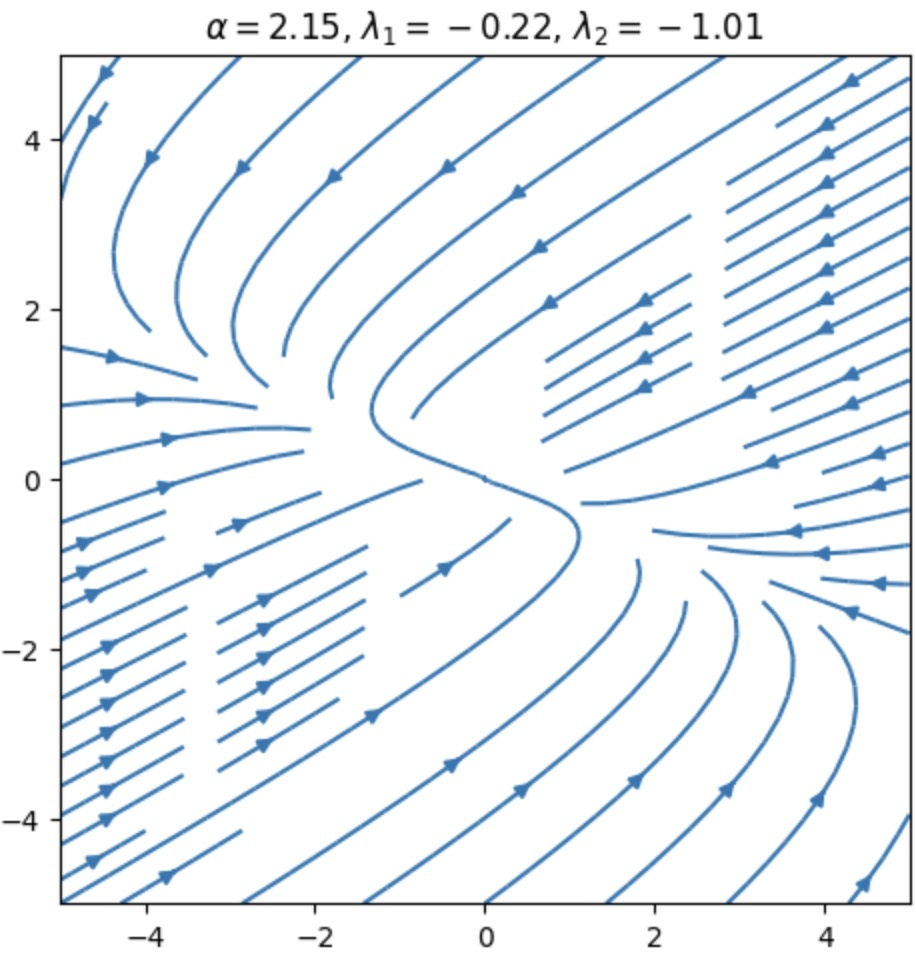
\includegraphics[width=0.18\textwidth]{images/stable_node.jpg}}
    \subfloat[\centering Stable focus]{
    \label{stable_focus}
    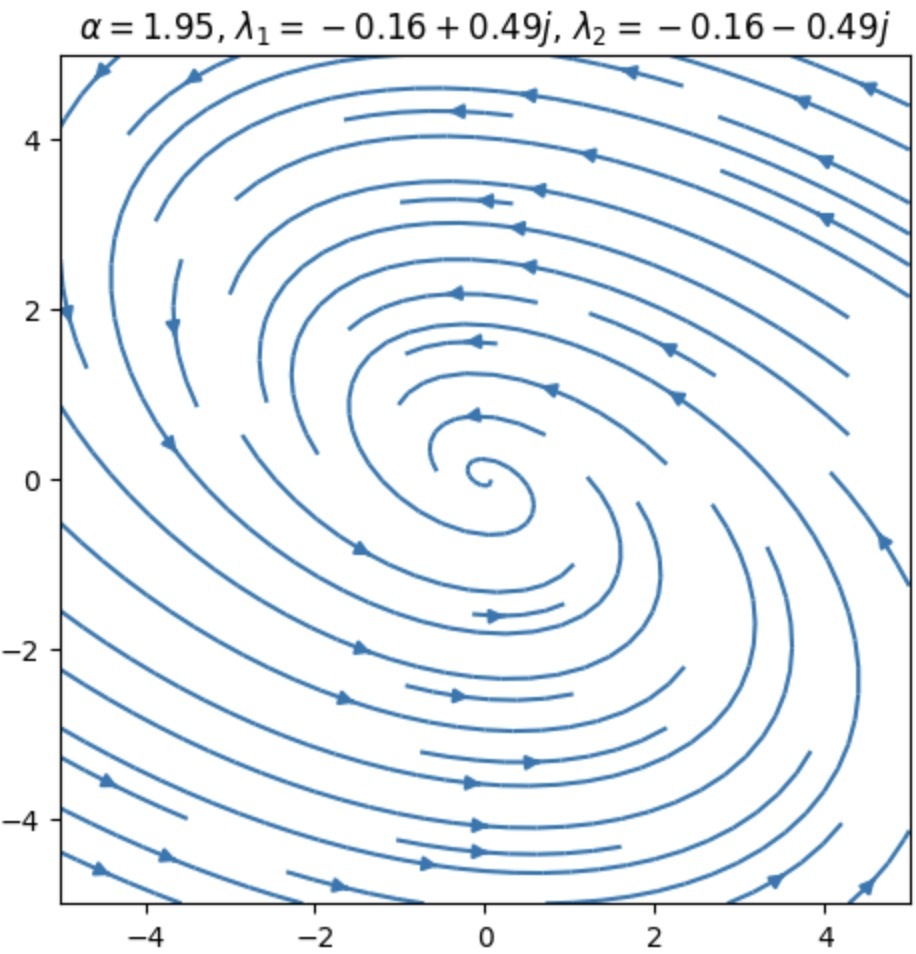
\includegraphics[width=0.18\textwidth]{images/stable_focus.jpg}}
    \subfloat[\centering Saddle]{
    \label{saddle}
    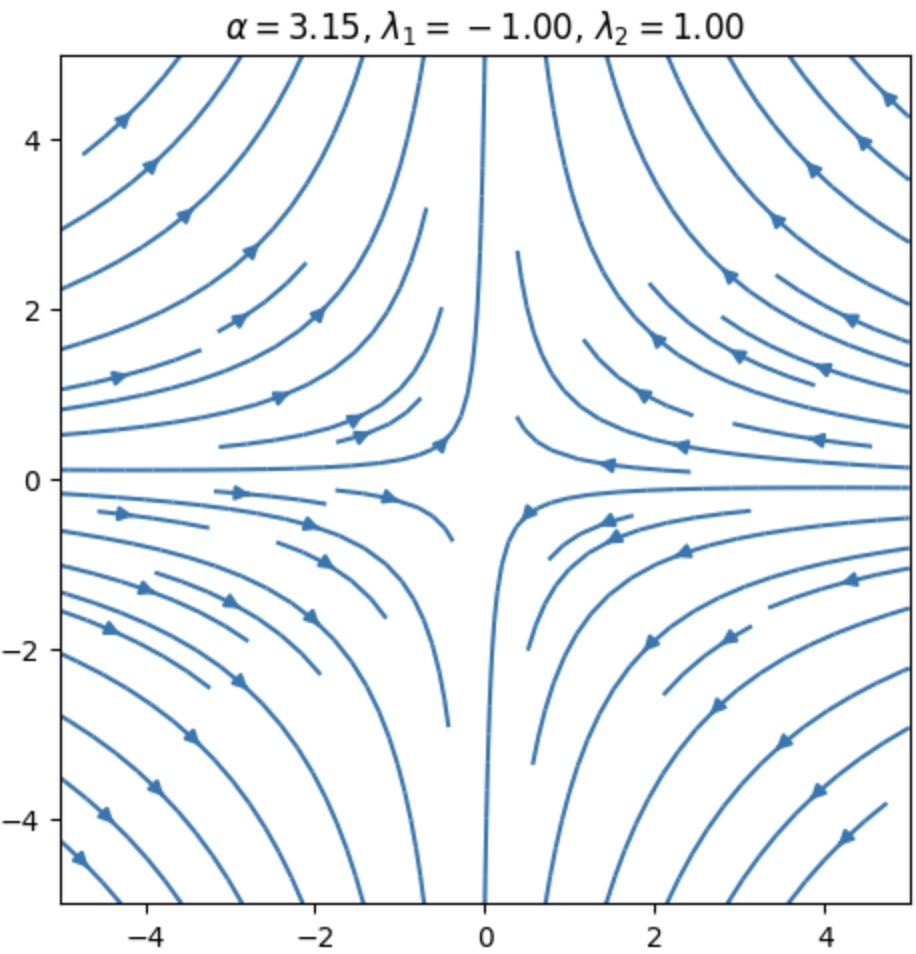
\includegraphics[width=0.18\textwidth]{images/saddle.jpg}}
    \subfloat[\centering Unstable node]{
    \label{unstable_node}
    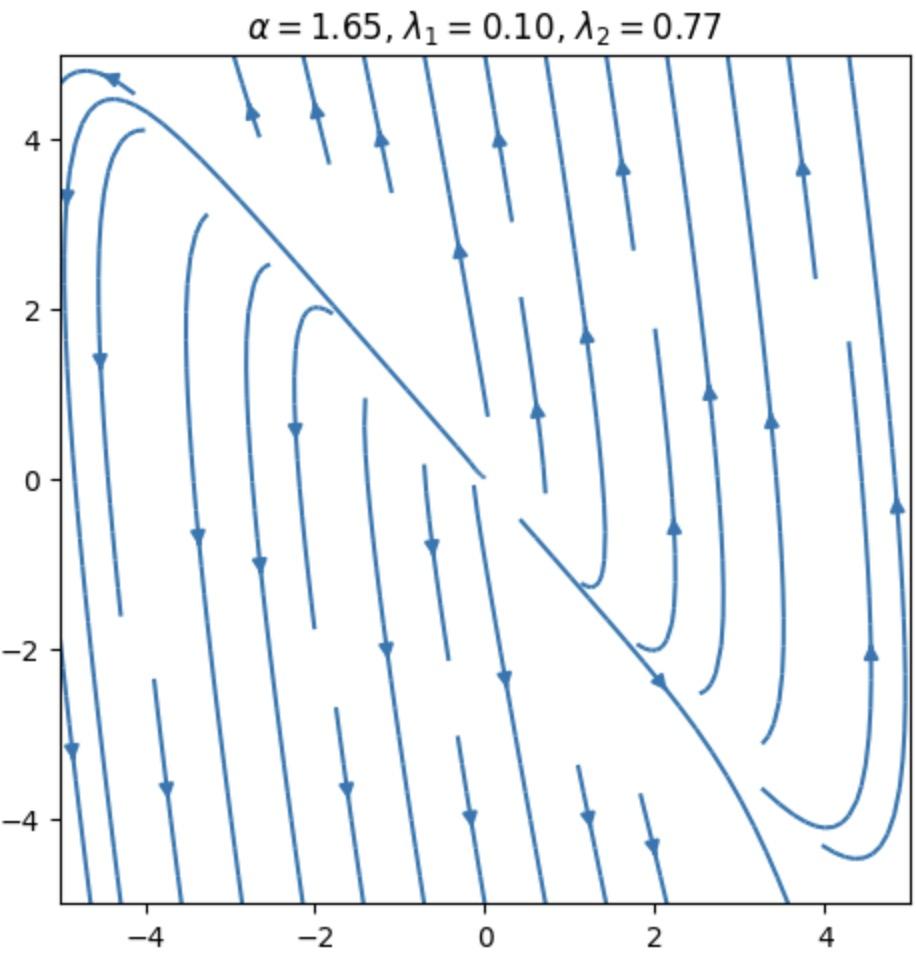
\includegraphics[width=0.18\textwidth]{images/unstable_node.jpg}}
    \subfloat[\centering Unstable focus]{
    \label{unstable_focus}
    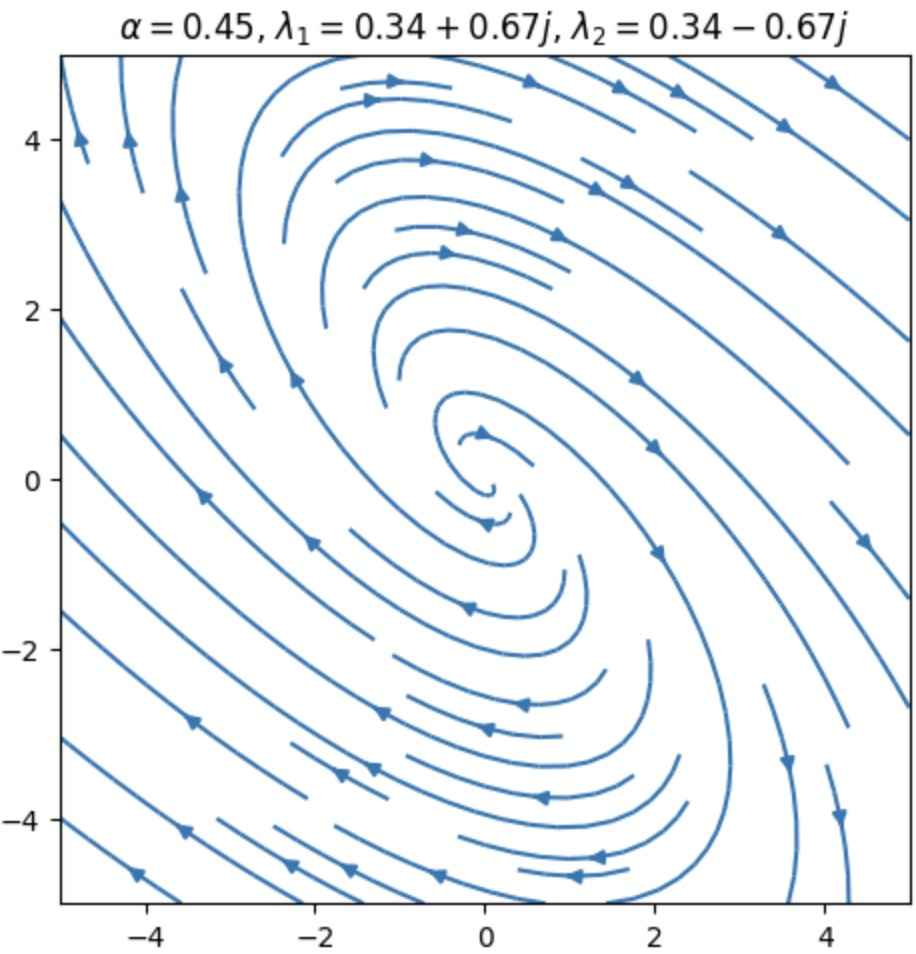
\includegraphics[width=0.18\textwidth]{images/unstable_focus.jpg}}
    \caption{Phase portraits of hyperbolic equilibria on the plane.}
    \label{phase_portraits}
\end{figure}

Figure \ref{phase_portraits} displays the different phase portraits of the three topological classes of hyperbolic equilibria, labeled accordingly with its class and the defined matrix $A_{\alpha}$ used to produce it. As stated in Kuznetsov's book, nodes and foci of corresponding stability are locally topologically equivalent within $U$, where $U$ denotes a small neighborhood $U\subset\mathbb{R}^{n}$ near an equilibrium point $x_0$. Therefore, \ref{stable_node} and \ref{stable_focus} as well as \ref{unstable_node} and \ref{unstable_focus} are locally topologically equivalent within $U$, while \ref{saddle} is not equivalent to any of the others.

\end{task}

\newpage

\begin{task}{2, Common bifurcations in nonlinear systems}

In the second task, we have to analyse the bifurcations in nonlinear systems. The notebook \texttt{Task2.ipynb} has been setup to construct the bifurcations diagrams, which essentially calls the \texttt{bifurcation\_diagram} function of \texttt{utils.py}. 

The two nonlinear dynamical system we have to analyse is described on the real line $X=\mathbb{R}$, $I=\mathbb{R}$. 

\noindent The first one with the following evolution equation: 

\begin{equation}\label{X}
    \dot{x} = {\alpha} - x ^2
\end{equation}

In the Figure \ref{function1} we can observe the plot of the bifurcation diagram of the system with the parameter $\alpha$ in the range of [-1, 1].

\begin{figure} [H]
    \centering
    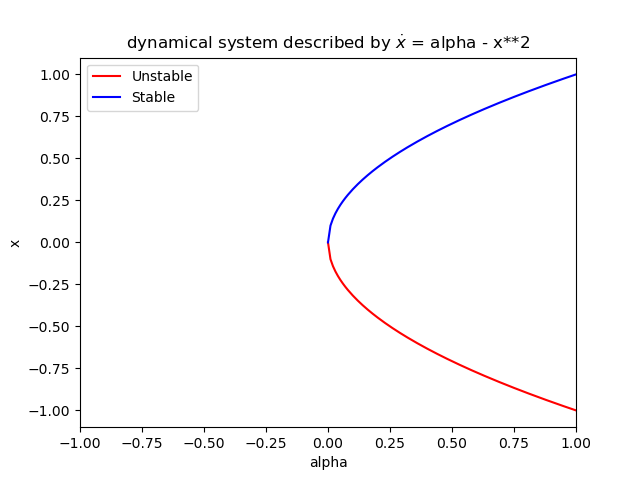
\includegraphics[width=15cm]{images/function1_task_2.png}
    \caption{Bifurcation diagram of the system described by $\dot{x} = {\alpha} - x ^2$}
    \label{function1}
\end{figure}

At ${\alpha} = 0$, there is only one equilibrium (or bifurcation) point, which is ${x_0} = 0$. For $\alpha > 0$ it has 2 equilibrium points (${x_0} = \pm \sqrt{\alpha}$, one stable and the other unstable) and there are no equilibrium points for $\alpha < 0$. It is a saddle-node bifurcation, one of the equilibrium points for $\alpha > 0$ is attractive and the other one is repulsive. It can be observed in the bifurcation diagram of the Figure \ref{function1}, where the red points are repulsive (unstable) and the blue points are attractive (stable).

\newpage

\noindent And the second one is described by the following evolution equation:

\begin{equation}\label{X2}
    \dot{x} = {\alpha} - 2x^2 - 3
\end{equation}

The next figure is the bifurcation diagram of the system with the parameter ${\alpha}$ in the range of [-20, 20].  

\begin{figure} [H]
    \centering
    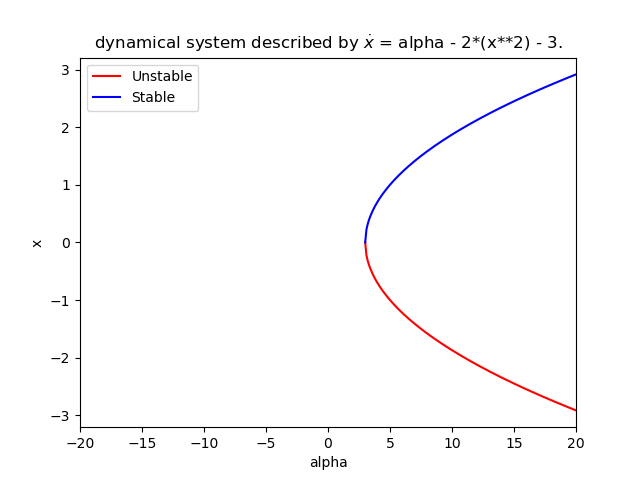
\includegraphics[width=15cm]{images/function2_task_2.png}
    \caption{Bifurcation diagram of the system described by $\dot{x} = {\alpha} - 2x^2 - 3$}
    \label{function2}
\end{figure}

As we can observe, the diagram is very similar to the previous one. In contrast of the previous function, at $\alpha = 3$ is where there is only one equilibrium point, which is again ${x_0} = 0$. The type of bifurcation is also saddle-node with attractive (stable) and repulsive (unstable) points as we can observe in the Figure \ref{function2}.

Two systems that have different steady states cannot be topologically equivalent because it doesn't exist a continuous transformation that can match all the states of one of the systems to the another. 

In fact, in the page 37 in the book of Kuznetsov \cite{Yuri} does say: \emph{``Thus, we have to specify when we define two dynamical systems as being "qualitatively similar" or equivalent. Such a definition must meet some general intuitive criteria. For instance, it is natural to expect that two equivalent systems have the same number of equilibria and cycles of the same stability types. The "relative position" of these invariant sets and the shape of their regions of attraction should also be similar for equivalent systems."}

So the two systems described before are not topologically equivalent at $\alpha = 1$, because one of them have 2 steady states (the system \ref{X}) and the other does not have any (the system \ref{X2}). But they are topologically equivalent at $\alpha = -1$ because both of them have 0 steady states and they have the same normal form.

Finally, we have to discuss about why the systems have the same normal form. Just by looking at the bifurcation diagrams we can notice that the parabola of both are very similar and have a lot of common. First, let's remind that the normal form of a quadratic function is $a(x - h)^2 + k$. Then, let's see the normal forms of our systems:
\begin{itemize}
  \item Normal form of the 1st system: $-1(x - 0)^2 + 0$
  \item Normal form of the 2nd system: $-2(x - 0)^2 + (-3)$
\end{itemize} 

The parameter a defines the amplitude of the parabola, a higher absolute value of a makes the parabola narrower and a small absolute value of a makes it wider. Just looking at the plots of the system before, we cannot appreciate it since they are in different ranges. So, we have create the bifurcation diagram of the first system in the range [-20, 20], so that we can see the difference. 
 
\begin{figure} [H]
    \centering
    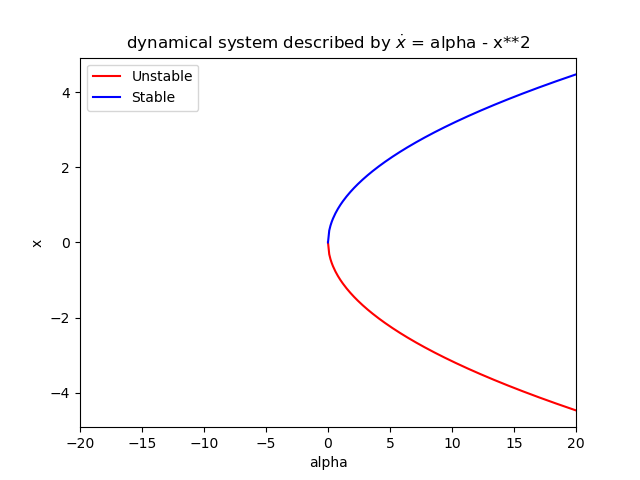
\includegraphics[width=15cm]{images/function1_2.png}
    \caption{Bifurcation diagram of the system described by $\dot{x} = {\alpha} - x ^2$ in [-20, 20]}
    \label{function1_2}
\end{figure}

As expected, if we compare the Figure \ref{function2} of the 2nd system with this figure of above of the first system, we can see that the parabola of the 1st system is the same of the other but just wider (between -4.5 and 4.5), the parabola of the 2nd system is between -3 and 3.

Then, let's talk about the other parameter: k. This just an offset parameter, it just moves the parabola to the left side or right side. We can see that the second system is just 3 more places (+3) to the right than the first one.

In conclusion, both have the same normal form and it is possible to obtain a mapping between the two dynamic systems by equalling the a and k parameters of their normal form.

\end{task}

\newpage

\begin{task}{3, Bifurcations in higher dimensions}

\noindent\textbf{Part 1}

The first part of this task asks to visualize the Andronov-Hopf bifurcation \cite[p.57]{Yuri}, which occurs in a two-dimensional state space $X=\mathbb{R}$ with one parameter $\alpha\in\mathbb{R}$, with the vector field in normal form

\begin{equation}
\begin{aligned}
    \dot{x}_1 &= \alpha {x_1} - x_2 - x_1 ({x_1^2} + {x_2^2}),\\
    \dot{x}_2 &= x_1 + \alpha x_2 - x_2 ({x_1^2} + {x_2^2}).
\end{aligned}
\end{equation}

To do so, the method shown in Listing \ref{system} has been implemented, which plots the vector field of the given system with the specified parameter $\alpha$. Thoroughly, it first initializes a grid and, for every point $(x, y)$ in it alongside the given $\alpha$, it evaluates the system and saves the resulting vectors for displaying them later on with the \texttt{streamplot()} method.

\begin{lstlisting}[language = Python, caption={Method for plotting the vector field of a two-dimensional system}, label={system}]
def phase_portrait_system(system: list, alpha: float):
    """
    Plots the phase portrait of the given 'system'
    :param system: two dimensional system ODEs
    :param alpha: system's parameter
    """
    w = 3
    Y, X = np.mgrid[-w:w:100j, -w:w:100j]
    U, V = [], []
    for x2 in X[0]:
        for x1 in Y[:, 0]:
            u = eval(system[0])
            v = eval(system[1])
            U.append(u)
            V.append(v)
    U = np.reshape(U, X.shape)
    V = np.reshape(V, X.shape)
    
    fig = plt.figure(figsize=(5, 5))

    ax0 = fig.add_subplot()
    ax0.streamplot(X, Y, U, V, density=2)
    ax0.set_aspect(1)
    ax0.set_title(r'$\alpha={0:.2f}$'.format(alpha))
    return ax0
\end{lstlisting}

Three phase diagrams at representative values of $\alpha$ can be visualized in Figure \ref{andronov-hopf}. For negatives values of $\alpha$ there is an attracting steady state at point $x_0 = (0, 0)$ and, as it approaches to positive values, the steady state bifurcates into a limit circle with radius $r = \alpha$ from $x_0$ and a repelling steady state at $x_0$.

\begin{figure} [H]
    \centering
    \subfloat[]{
    \label{andronov-1}
    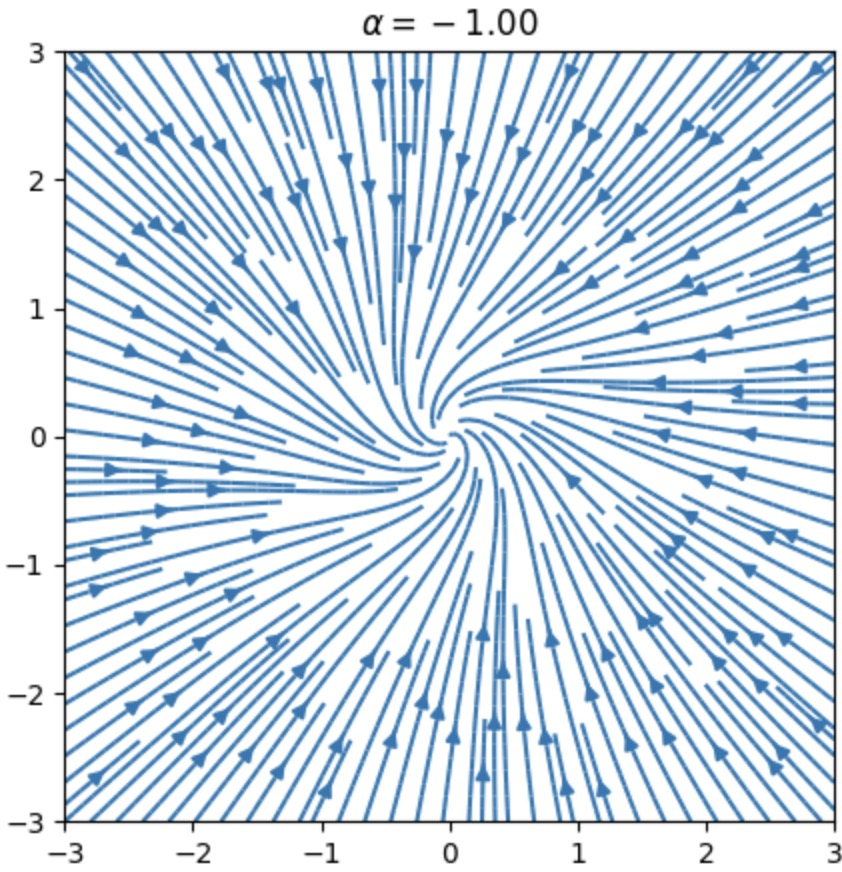
\includegraphics[width=0.25\textwidth]{images/andronov-1.jpg}}
    \subfloat[]{
    \label{andronov0}
    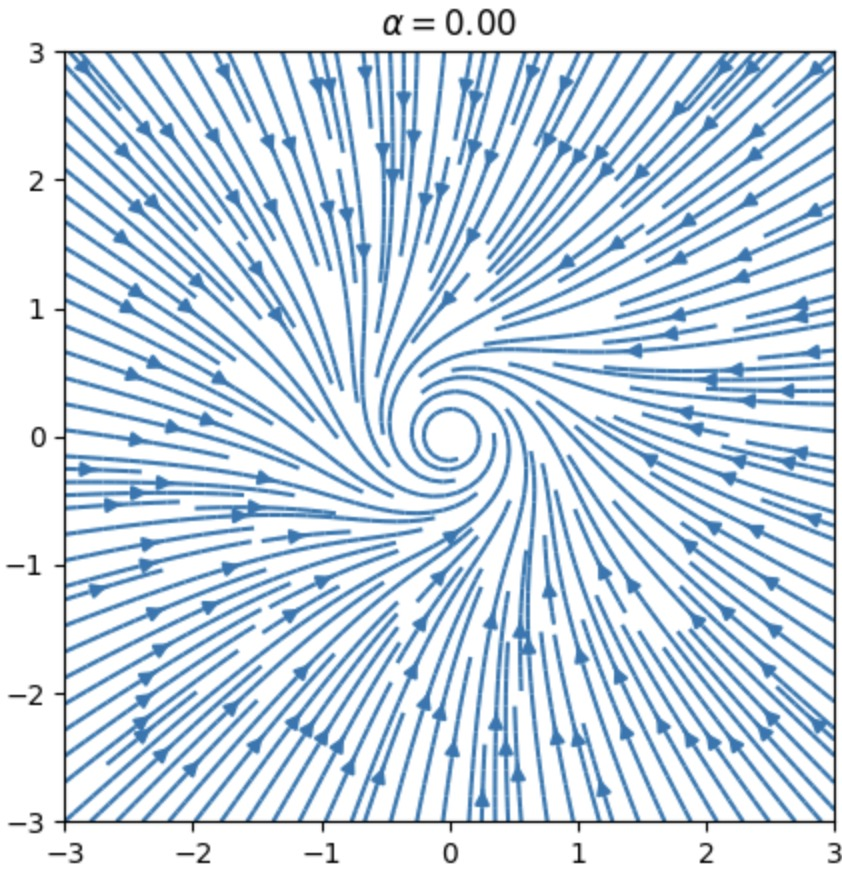
\includegraphics[width=0.25\textwidth]{images/andronov0.jpg}}
    \subfloat[]{
    \label{andronov1}
    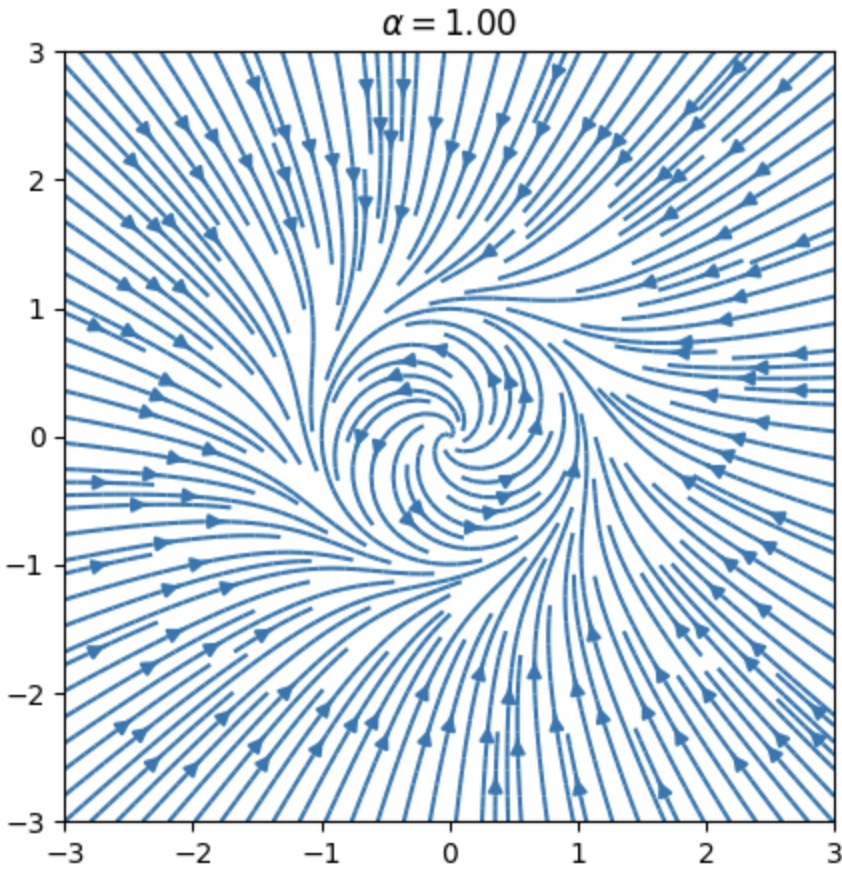
\includegraphics[width=0.25\textwidth]{images/andronov1.jpg}}
    \caption{Andronov-Hopf bifurcation with different $\alpha$ values.}
    \label{andronov-hopf}
\end{figure}

\newpage

The method shown in Listing \ref{orbit_system} has been implemented for plotting orbits of a system forward in time. It uses Euler's method with a very small time step to compute the points of the orbit. Starting from a given point $y_0$, the next point is calculated by summing the vector obtained by evaluating both systems with the previous point and multiplying it by the step size.

\begin{lstlisting}[language = Python, caption={Method for plotting orbits of a system forward in time}, label={orbit_system}]
def solve_euler_system(system, alpha, y0, time):
    """
    Solves the given ODE system using forward Euler.
    :param system: system ODEs
    :param y0: the initial condition to start the solution at.
    :param time: np.array of time values (equally spaced), where the solution must be obtained.
    :returns: (solution[time,values], time) tuple.
    """
    yt = np.zeros((len(time), len(y0)))
    yt[0, :] = y0
    step_size = time[1]-time[0]
    for k in range(1, len(time)):
        x1 = yt[k-1,0]
        x2 = yt[k-1,1]
        u = eval(system[0])
        v = eval(system[1])
        yt[k, :] = yt[k-1, :] + step_size * np.array([u, v])
    return yt, time
\end{lstlisting}

The behaviour of the orbits of the system forward in time is represented in Figure \ref{orbits}. As seen in Figures \ref{orbit1} and \ref{orbit2}, orbits starting inside and outside the limit circle will be repelled and attracted, respectively, until they reach the limit circle. Once an orbit reaches the limit circle, it adopts a counterclockwise oscillatory motion.

\begin{figure} [H]
    \centering
    \subfloat[$y_0=(0.5, 0)$]{
    \label{orbit1}
    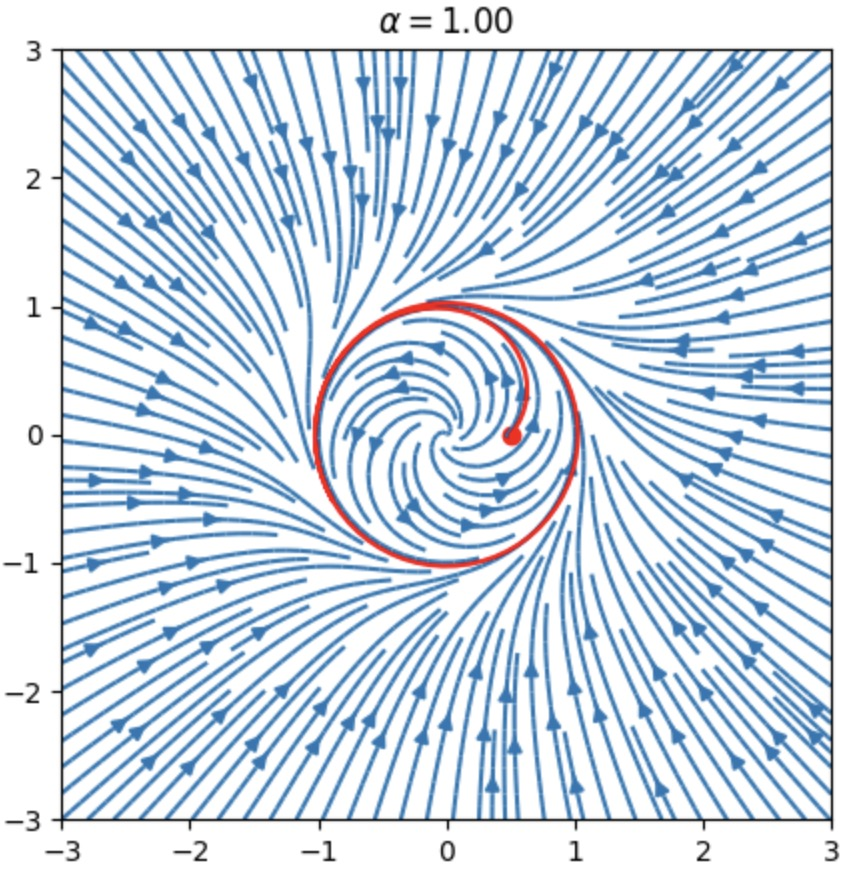
\includegraphics[width=0.25\textwidth]{images/orbit2.jpg}}
    \subfloat[$y_0=(1, 0)$]{
    \label{orbit3}
    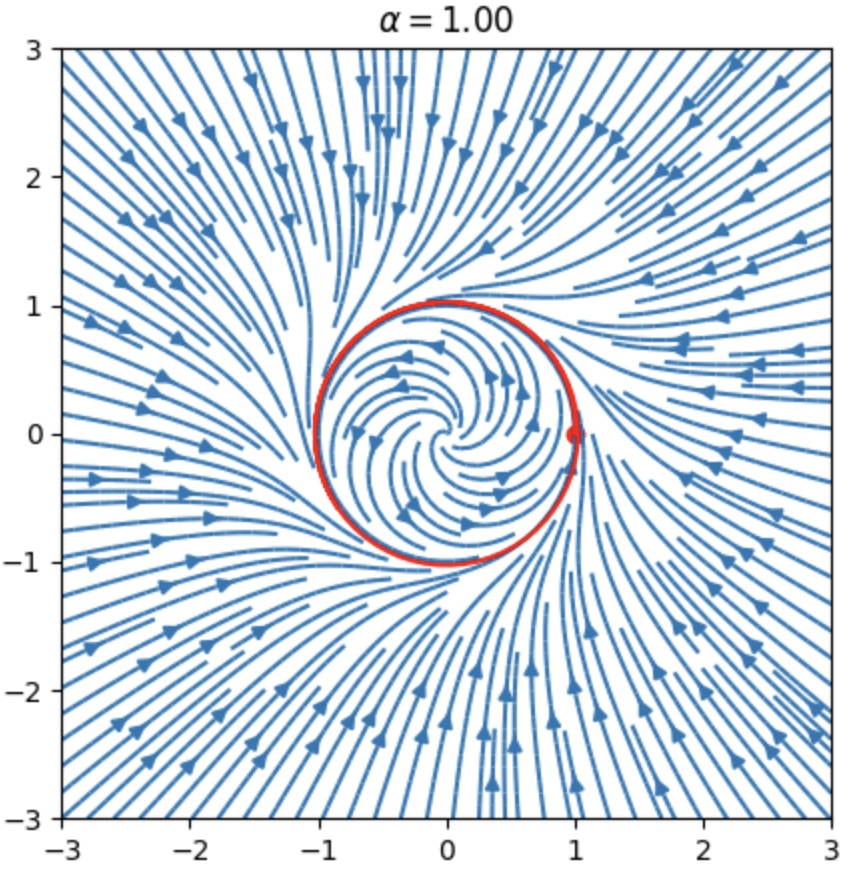
\includegraphics[width=0.25\textwidth]{images/orbit3.jpg}}
    \subfloat[$y_0=(2, 0)$]{
    \label{orbit2}
    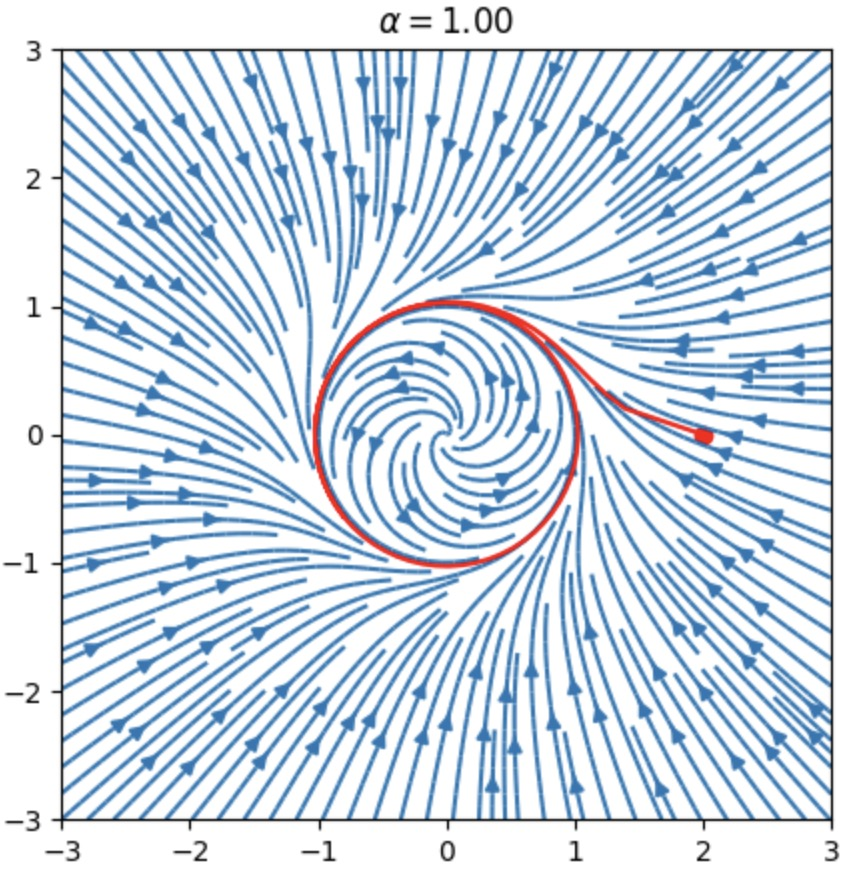
\includegraphics[width=0.25\textwidth]{images/orbit1.jpg}}
    \caption{Three orbits of the system forward in time for $\alpha=1$, starting at different points $y_0$.}
    \label{orbits}
\end{figure}

\noindent\textbf{Part 2}

The second part is about the cusp bifurcation, which occurs in one state space dimension $X=\mathbb{R}$ with two parameters $\alpha\in\mathbb{R}^2$, with normal form

\begin{equation}
    \dot{x} = \alpha_1 + \alpha_2 x - x^3.
\end{equation}

The setup for plotting the cusp bifurcation is shown in Listing \ref{cusp_method}. This method samples points $(x, \alpha_2)$ uniformly and calculates $\alpha_1$ as a function of $(x, \alpha_2)$. Since for some points $(\alpha_1, \alpha_2)$ it can exist more than one solution $x$, i.e. there is more than one steady state and therefore a bifurcation occurs, for every $\alpha_1$ calculated, the $x$ value is saved for its corresponding point $(\alpha_1, \alpha_2)$. This will be useful for plotting the 2D diagram later on, which given the surface defined by $\alpha_1$ and $\alpha_2$, scatters with a different color those points that have more than one fixed point $x$.

\newpage

\begin{lstlisting}[language = Python, caption = {Method for visualizing the cusp bifurcation in a 3D and 2D plot.}, label = {cusp_method}]
def cusp_bifurcation():
    """
    Creates 3D and 2D plots of the cusp bifurcation 
    """
    # Sample (x, a2) uniformly
    a2_samples = [round(a2, 2) for a2 in np.random.uniform(0, 1.5, 50000)]
    x_samples = [round(x, 2) for x in np.random.uniform(-1.5, 1.5, 50000)]
    a1_samples = []
    solutions = {}
    for x, a2 in zip(x_samples, a2_samples):
        # Calculates a1 for every (x, a2)
        a1 = round(-a2 * x + x ** 3, 2)
        a1_samples.append(a1)
        
        # Keeps records of x for every (a1, a2)
        key = (a1, a2)
        if key in solutions:
            solutions[key].add(x)
        else:
            solutions[key] = {x}
    
    def create_axes(angle1, angle2, position):
        """
        Adds a 3D subplot to a figure given the angles of visualization and the position
        This subplot scatters the different samples 'a1_samples', 'a2_samples' and 'x_samples'
        :param angle1: first angle of visualization
        :param angle2: second angle of visualization
        :param position: position of the subplot in the figure
        """
        ax = fig.add_subplot(1, 3, position, projection='3d')
        ax.scatter(a1_samples, a2_samples, x_samples, cmap = "viridis", c = a2_samples)
        ax.set_xlabel(r'$\alpha_1$')
        ax.set_ylabel(r'$\alpha_2$')
        ax.set_zlabel(r'$x$')
        ax.view_init(angle1, angle2)
        return ax
    
    # 3D plot
    fig = plt.figure(figsize=plt.figaspect(0.3))
    ax1 = create_axes(-90, 90, 1)
    ax2 = create_axes(120, -90, 2)
    ax3 = create_axes(-120, 90, 3)
    plt.show()
    
    # 2D plot
    fig = plt.figure()
    # Creates a colormap for every point (a1, a2)
    # If it has more than one solution x, a red point will be plotted, blue otherwise
    colors = ["red" if len(solutions[(a1, a2)]) > 1 else "blue" for a1, a2 in zip(a1_samples, a2_samples)]
    ax2d = plt.axes()
    ax2d.set_xlabel(r'$\alpha_1$')
    ax2d.set_ylabel(r'$\alpha_2$')
    ax2d.scatter(a1_samples, a2_samples, s=1, c=colors)
    plt.show()
\end{lstlisting}

\newpage

The equilibrium manifold near the cusp bifurcation is shown in Figure \ref{3dcusp} with different angles of view. Citing from \cite{Cusp}, \emph{``At the cusp bifurcation point two branches of saddle-node bifurcation curve meet tangentially, forming a semicubic parabola. For nearby parameter values, the system can have three equilibria which collide and disappear pairwise via the saddle-node bifurcations. The cusp bifurcation implies the presence of a hysteresis phenomenon."}

\begin{figure} [H]
    \centering
    \subfloat[]{
    \label{cusp1}
    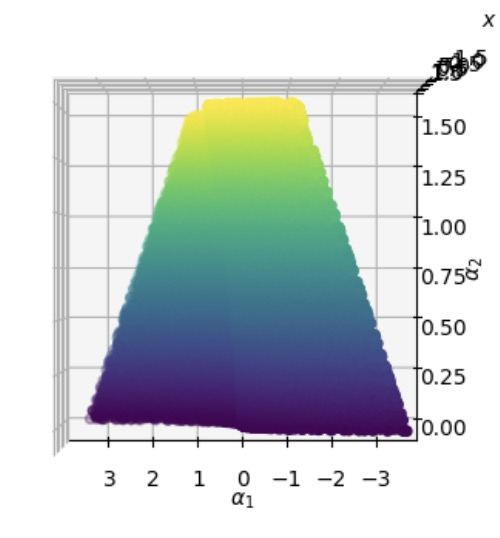
\includegraphics[width=0.25\textwidth]{images/cusp1.jpg}}
    \subfloat[]{
    \label{cusp2}
    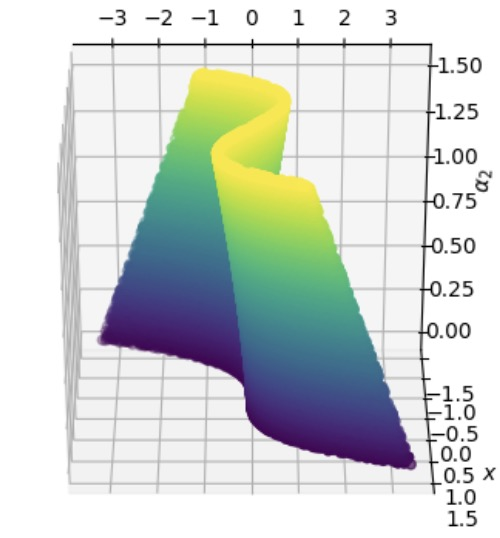
\includegraphics[width=0.25\textwidth]{images/cusp2.jpg}}
    \subfloat[]{
    \label{cusp3}
    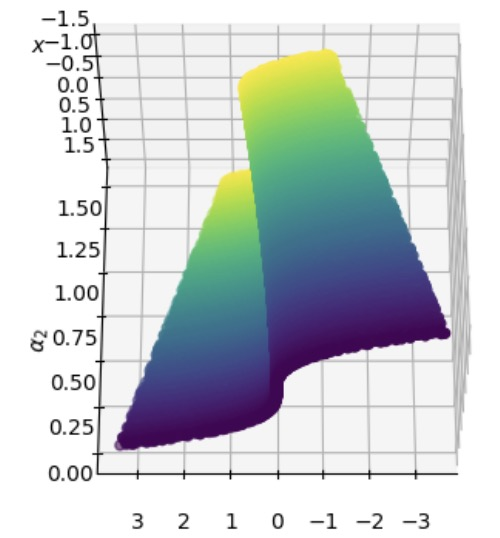
\includegraphics[width=0.25\textwidth]{images/cusp3.jpg}}
    \caption{Bifurcation surface of the cusp bifurcation in a 3D plot with different angles of view.}
    \label{3dcusp}
\end{figure}

A more intuitive vision of the cusp form can be seen in the 2D projection of the surface given by $\alpha_1$ and $\alpha_2$, displayed in Figure \ref{2dcusp}. Points where there are more than one steady state are colored in red, whereas those with only one are colored in blue. The cusp form is clearly defined in the red area, even though there is some noise due to the precision rounding.

\begin{figure}[H]
    \centering
    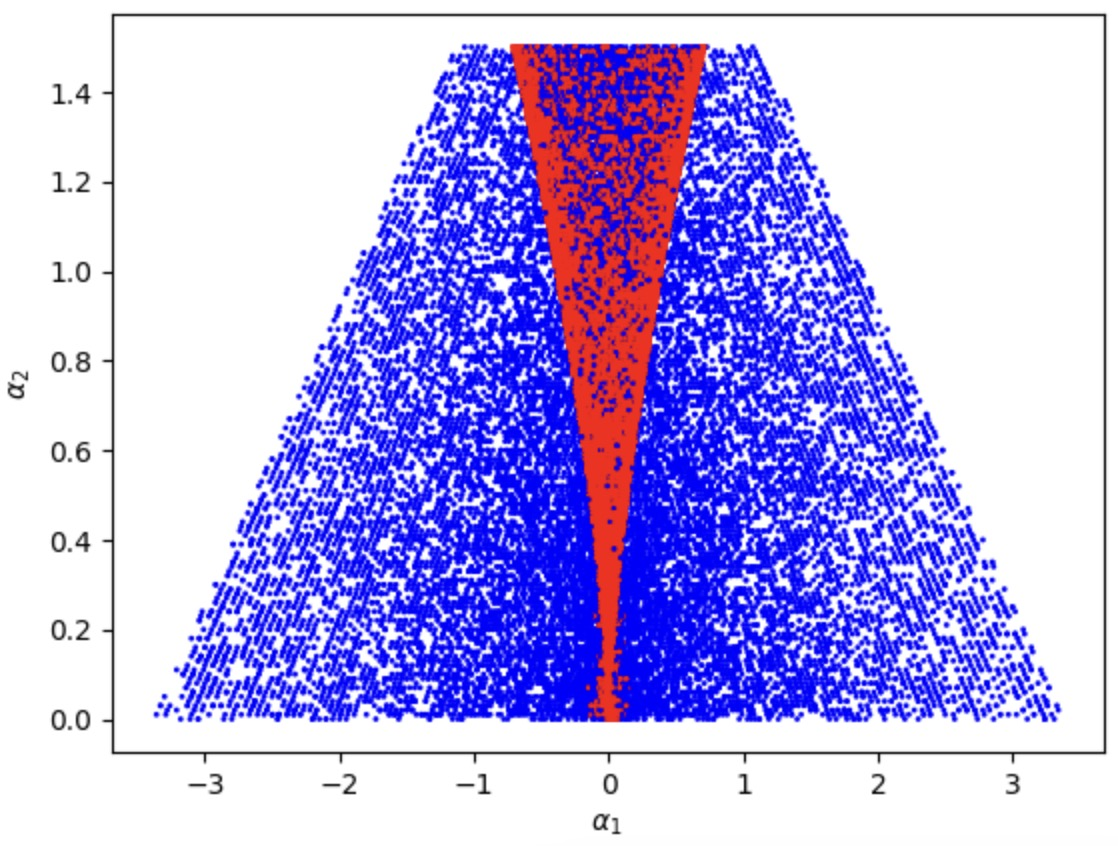
\includegraphics[width=6cm]{images/cusp2d.jpg}
    \caption{Bifurcation surface of the cusp bifurcation in a 2D plot.}
    \label{2dcusp}
\end{figure}

\end{task}

\newpage

\begin{task}{4, Chaotic dynamics}

\bigskip
Dynamical systems can behave in very irregular ways, and changes in their parameters can lead to very drastic changes in their behavior. In this task, we study two renowned dynamical systems: the logistic map and the Lorenz attractor.

\bigskip
\noindent \textbf{Part 1:}

The logistic map is a discrete-time demographic function used to model population growth, which can be defined numerically as 
\begin{equation}
    x_{n+1}=rx_n(1-x_n), n\in \mathbb{N}
\end{equation}
in which $x_n$ is the population at time $n$, and $r\in (0,4]$ is a parameter that determines the rate of growth. For certain values of $r$, the logistic map exhibits chaotic behavior.

\begin{lstlisting}[language = Python,  label = {cusp_method}]
def logistic_map(x, rate):
    '''
    Definition of the equation for the logistic map.
    :param x: float
        current population value at time t
    :param rate: float
        growth rate parameter values
    :returns: float
        scalar result of logistic map at time t+1
    '''
    return rate * x * (1 - x)
\end{lstlisting}

To simplify the calculation and visualization process, we implemented our functions, taking reference from several popular tools used in the field of dynamical systems in mathematics for iterative discrete functions, to simulate and display the function results simultaneously in the form of series plot, cobweb plot (Verhulst diagram) and bifurcation plot. 

\begin{lstlisting}[language = Python, label = {cusp_method}] 
def get_function_points(model, r, n, start, end):
    '''
    Calculate the model results x_{i+1} for n x_i values evenly spaced between [start, end] period.
    :param model: function
        a defined iterated map to simulate
    :param r: float
        growth rate parameter value to pass to the map function
    :param n: int
        number of different x_i to space and calculate
    :param start: float
        lower limit of the function range
    :param end: float
        upper limit of the function range
    :returns: tuple
        x_vals, y_vals: tuple of the x_i series and its corresponding x_{i+1} values
    '''
    x_vals = np.linspace(start, end, n)
    y_vals = [model(x, r) for x in x_vals]
    return x_vals, y_vals

def get_cobweb_points(model, r, x, n):
    '''
    Based on pynamical `https://github.com/gboeing/pynamical`
    Calculate the vertices of cobweb lines for a cobweb plot.

    Steps in the calculation:
    1) Let x = 0.5
    2) Start on the x-axis at the point (x, 0).
    3) Draw a vertical line to the red function curve: this point has the coordinates (x, f(x)).
    4) Draw a horizontal line from this point to the gray diagonal line: this point has the coordinates (f(x), f(x)).
    5) Draw a vertical line from this point to the red function curve: this point has the coordinates (f(x), f(f(x))).
    6) Repeat steps 4 and 5 recursively one hundred times.

    :param model: function
        a defined iterated map to simulate
    :param r: float
        growth rate parameter value to pass to the map function
    :param x: float
        starting population value
    :param n: int
        number of iterations to run
    :returns: tuple
        x0_vals, cobweb_y_vals: tuple of the iterated (x_i, x_{i+1}) position series
    '''
    cobweb_points = [(x, 0)]
    for _ in range(n):
        y1 = model(x, r)
        cobweb_points.append((x, y1))
        cobweb_points.append((y1, y1))
        y2 = model(y1, r)
        cobweb_points.append((y1, y2))
        x = y1
    return zip(*cobweb_points)
\end{lstlisting}

Cobweb plot is an auxiliary visualization tool for discrete function iterations, by calculating coordinates of the points on which for specific $x_0$ and $r$, we can efficiently retrieve information for both the series plot result of how $x_n$ value changes across time, and also the bifurcation plot result of the steady $x_\infty$ values for each $r$. And the bifurcation plot is a graphical representation of the behavior of the logistic map as the parameter $r$ varies, showing how the number and stability of the fixed points changes over time.

For better monitoring and demonstrating the results, in addition to plotting the above images, we also designed interactive interface to intuitively observe the effect of different $x_0$ and $r$ on the results in real time.

\begin{figure} [H]
    \centering
    \subfloat[$r=0.90$]{
        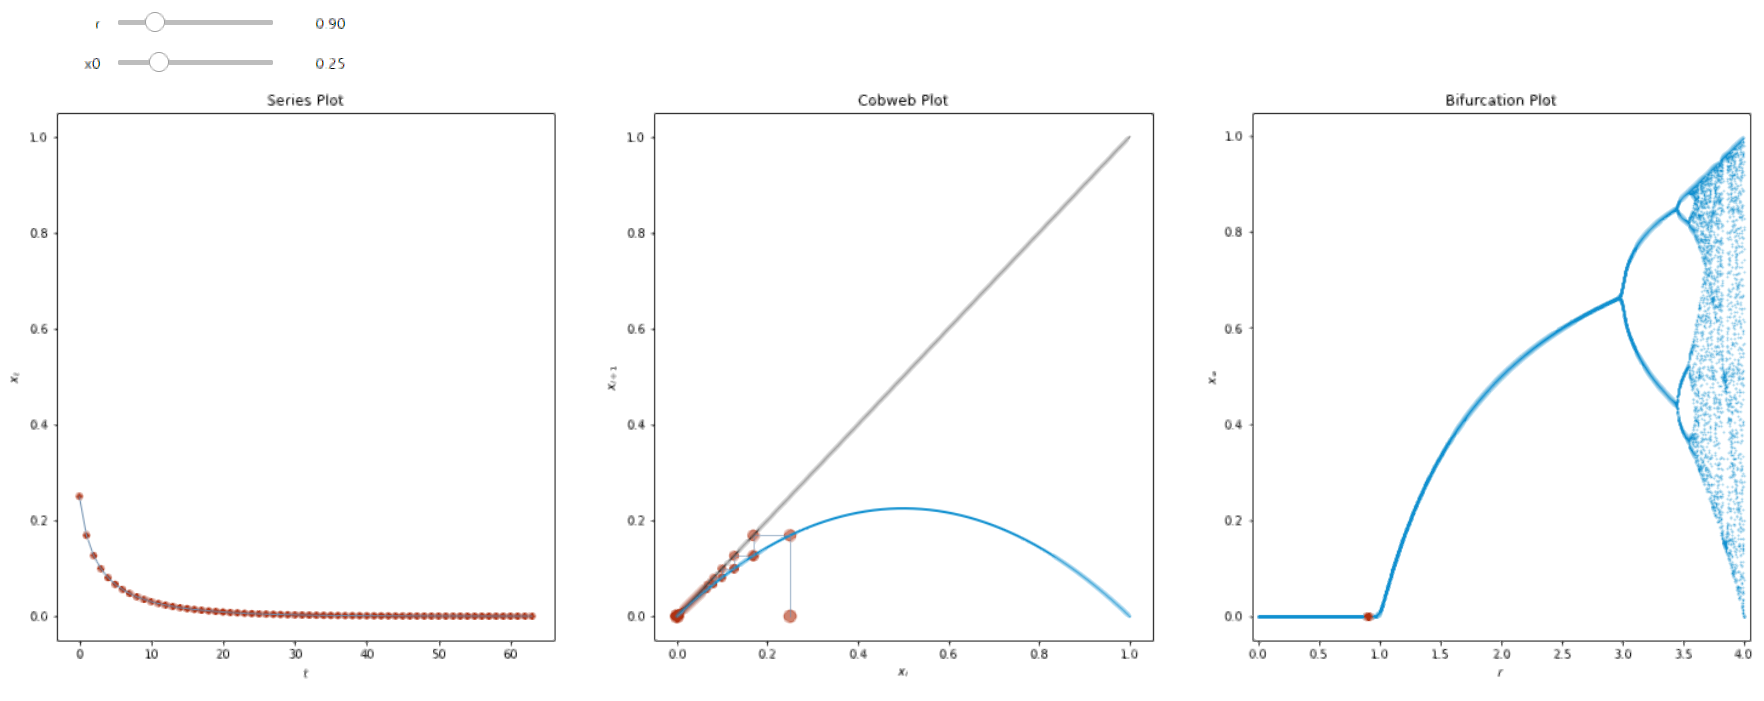
\includegraphics[width=.7\textwidth]{images/task4-1 (1).png}}
    \\
    \subfloat[$r=1.90$]{
        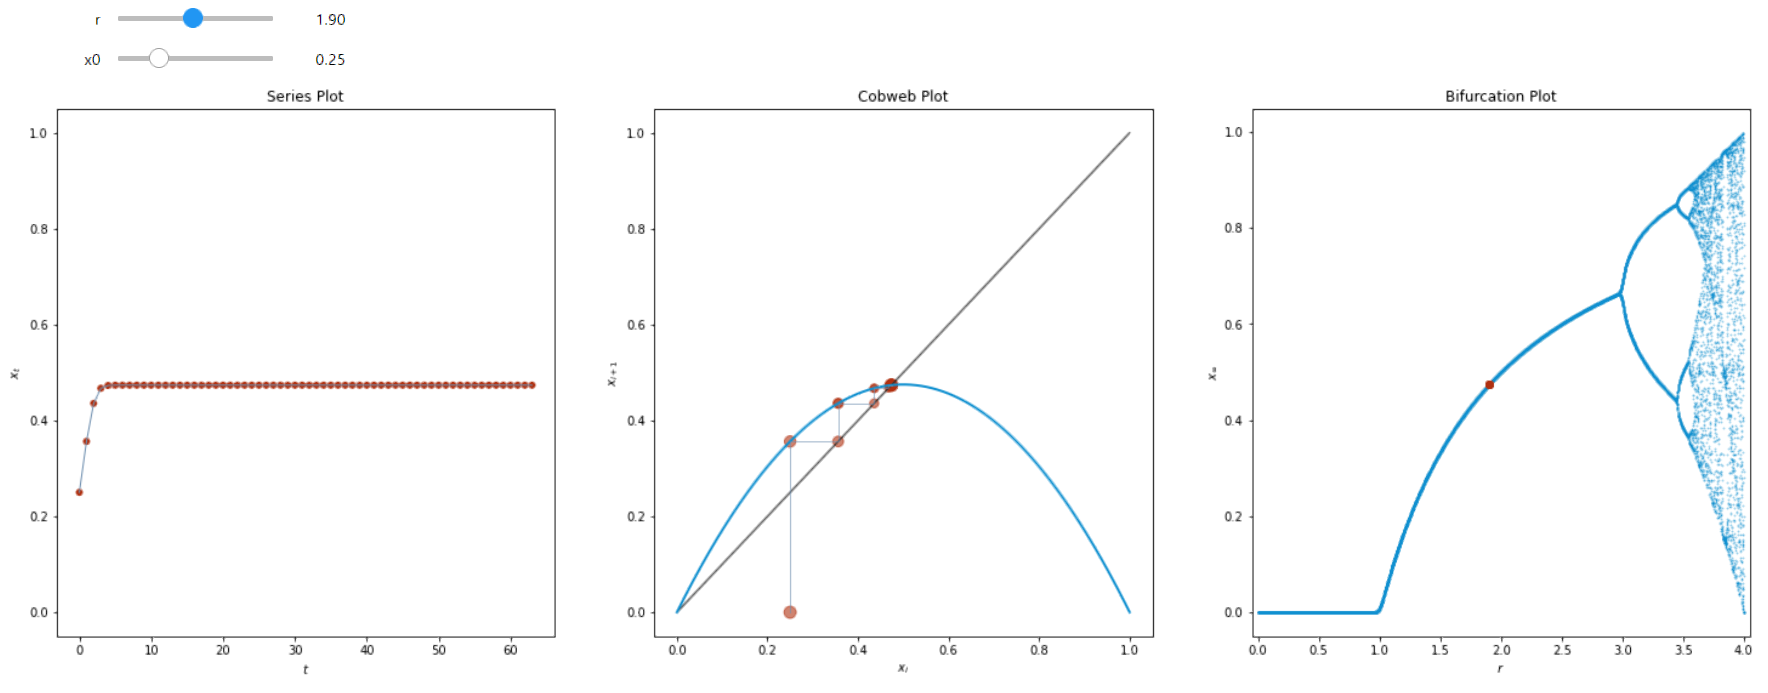
\includegraphics[width=.7\textwidth]{images/task4-1 (2).png}}
    \caption{Results of varying $r$ from 0 to 2, with $x_0=0.25$}
    \label{fig:task4-1-1}
\end{figure}

By varying $r$ from 0 to 2, we can observe that the stable state changes from convergence down to 0 to convergence to a specific value. Such bifurcation happens at $r=1$,  where the coordinates on the bifurcation plot changes from $x_\infty=0$ to $x_\infty=\frac{r-1}{r}$. This can also be interpreted by considering the practical implications of the model parameters, that $r$ represents the reproduction rate where the population will increase to the current population, and for $r\in (0,1)$ the population will eventually die, independent of the initial population, where with $r$ between 1 and 2 it will reach the environmental carrying capacity.

\begin{figure} [H]
    \centering
    \subfloat[$r=2.70$]{
        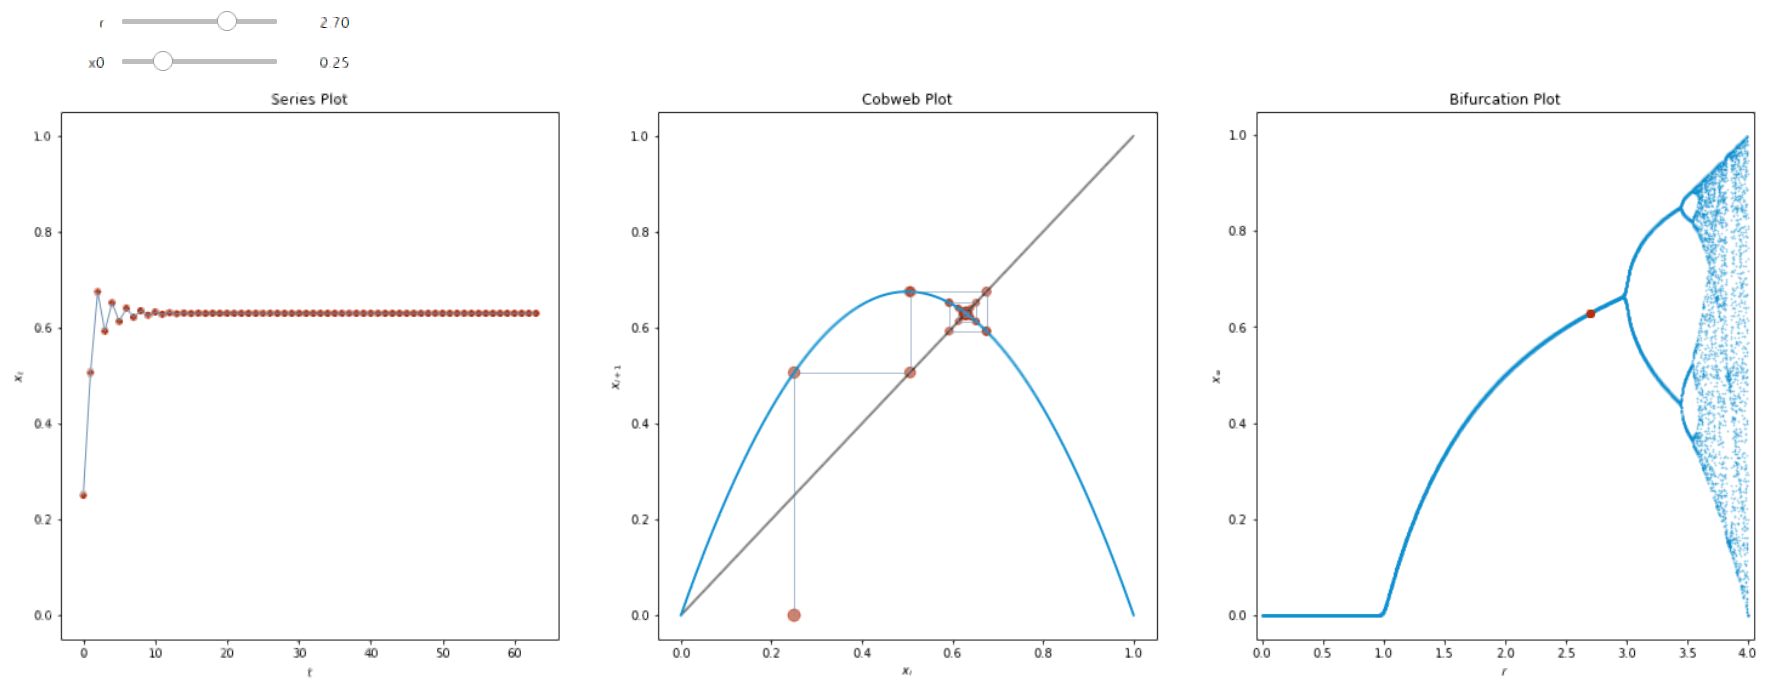
\includegraphics[width=.7\textwidth]{images/task4-1 (3).png}}
    \\
    \subfloat[$r=3.15$]{
        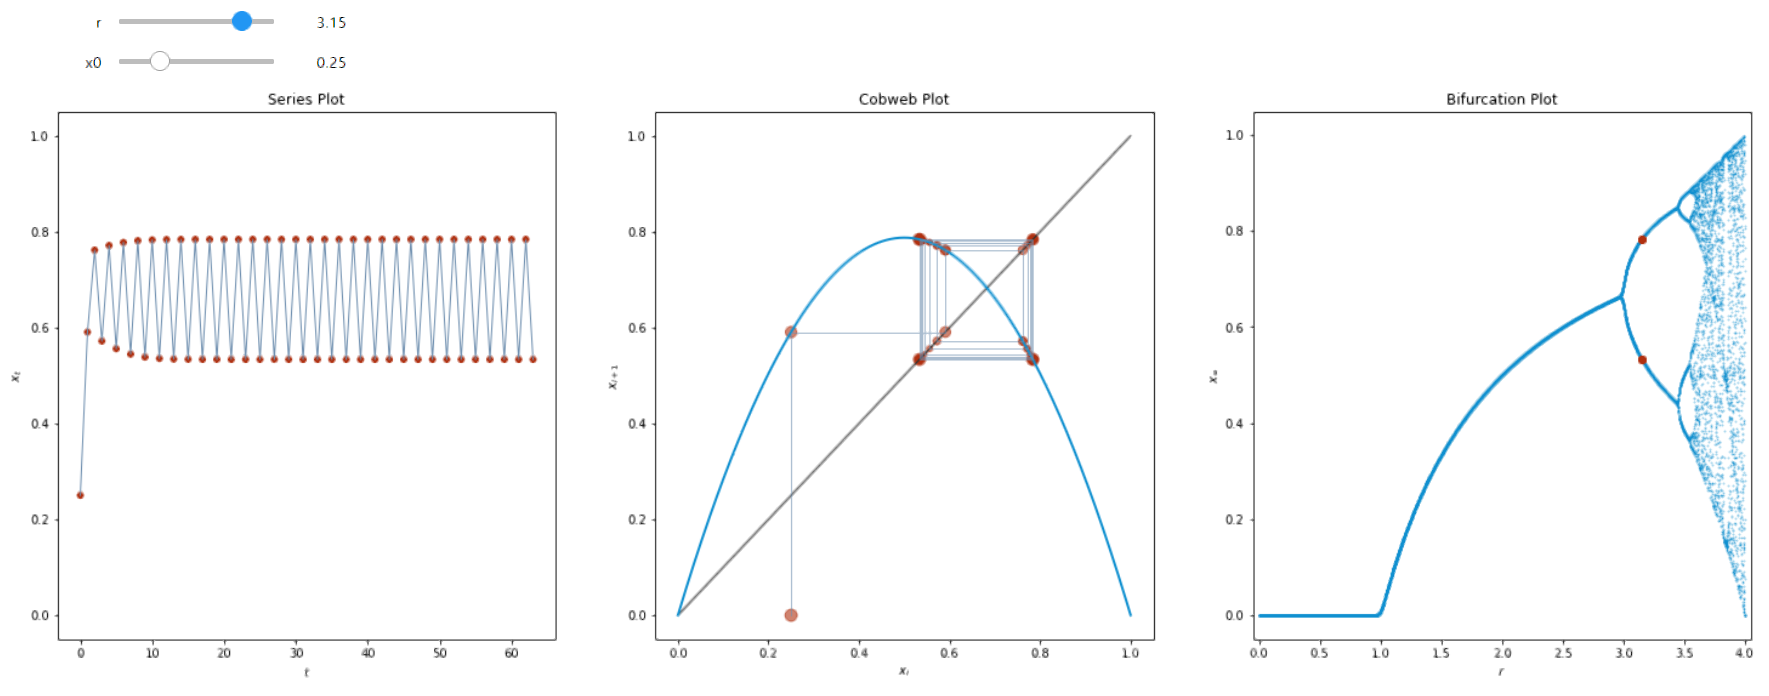
\includegraphics[width=.7\textwidth]{images/task4-1 (4).png}}
    \\
    \subfloat[$r=3.50$]{
        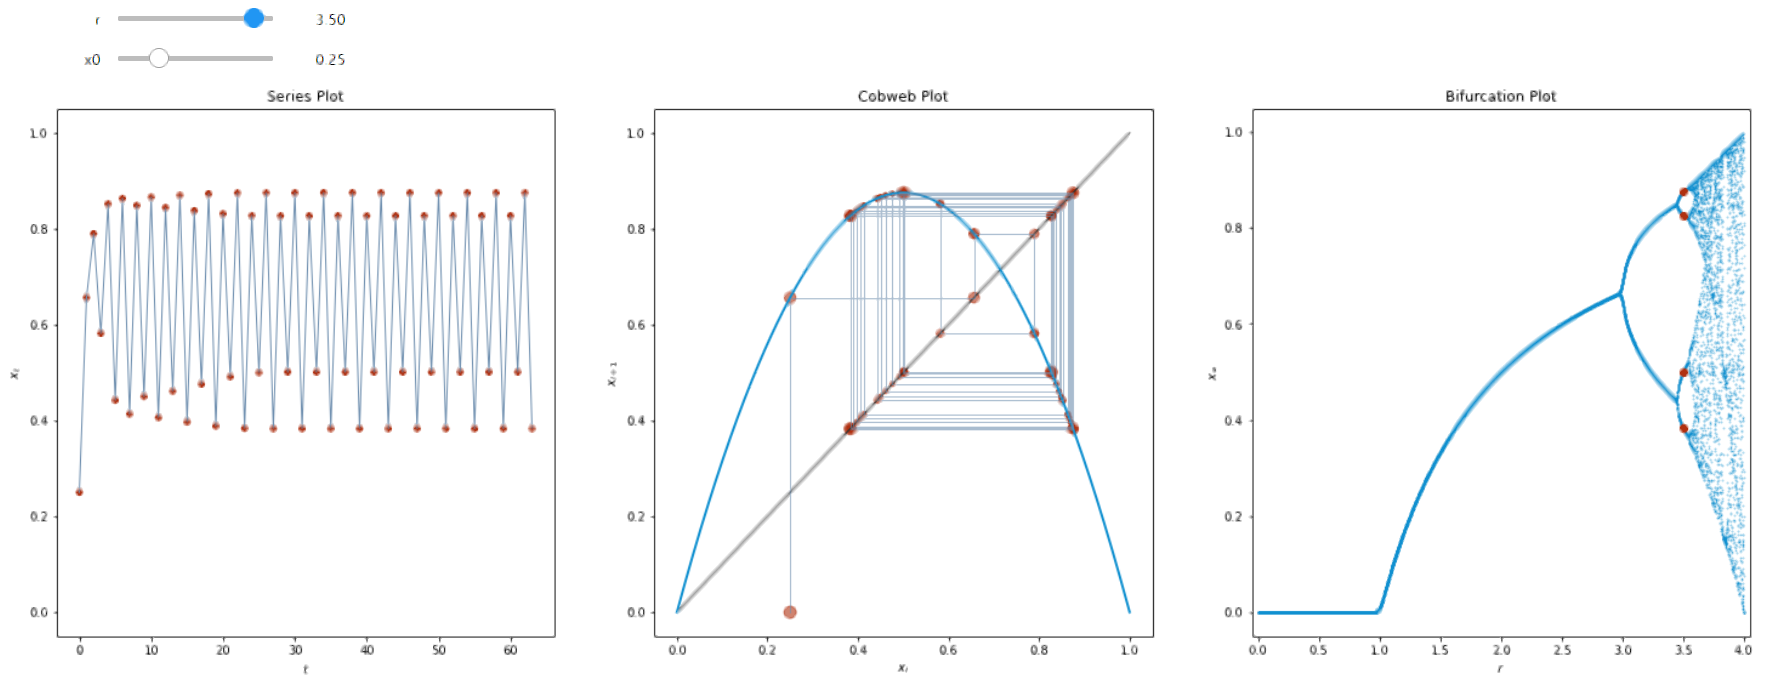
\includegraphics[width=.7\textwidth]{images/task4-1 (5).png}}
    \\
    \subfloat[$r=3.80$]{
        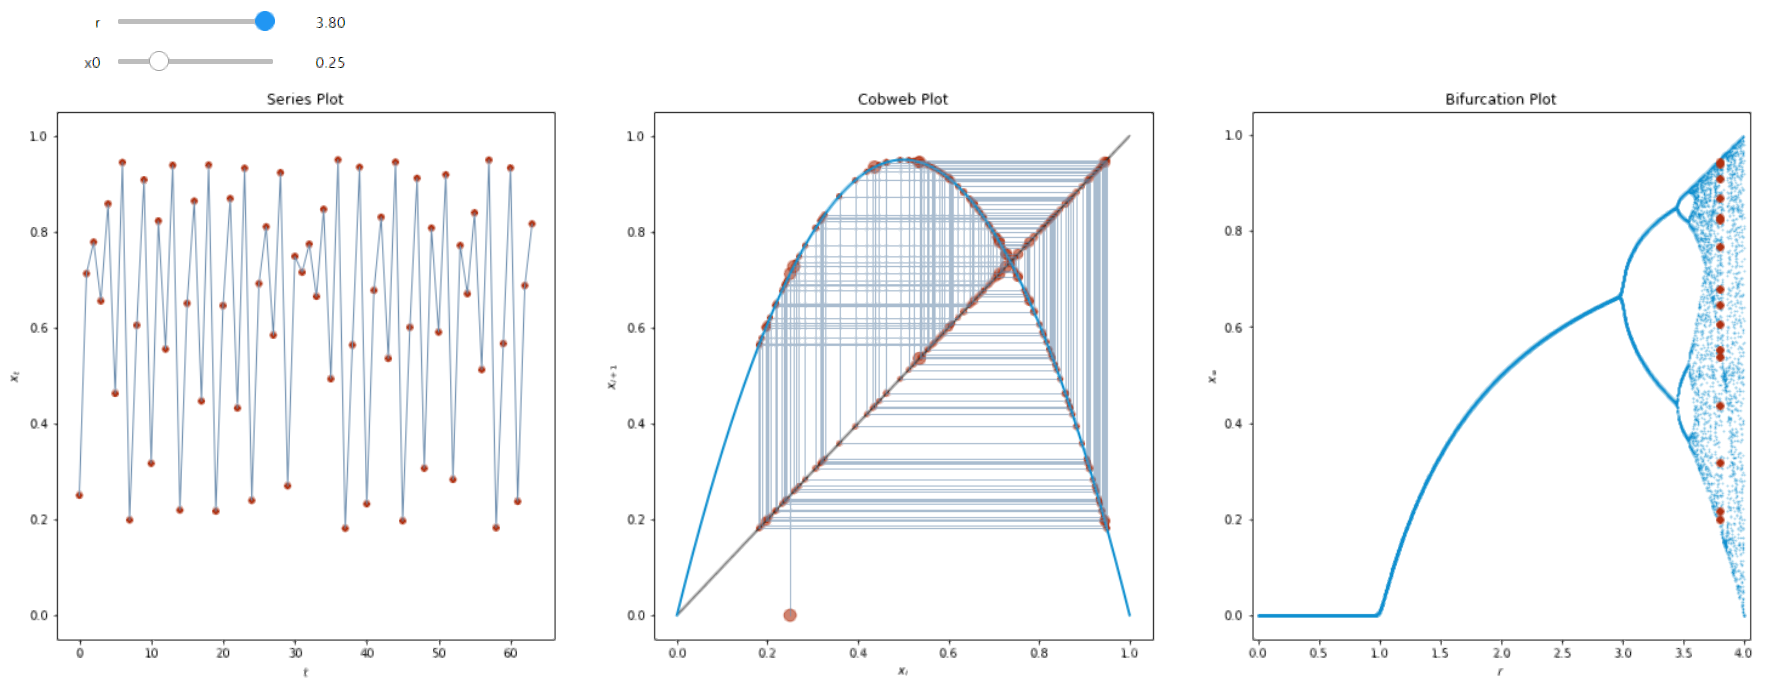
\includegraphics[width=.7\textwidth]{images/task4-1 (6).png}}
    \caption{Results of varying $r$ from 2 to 4, with $x_0=0.25$}
    \label{fig:task4-1-2}
\end{figure}

By varying $r$ from 2 to 3, we can observe that the state is still approaching the same $x_\infty=\frac{r-1}{r}$, whereas approaching from both side with decaying oscillations. And as $r$ getting closer to 3, the convergence get slower. With approximately $r\in(3, 3.44]$, the population will approach permanent oscillations between two values dependent on $r$, and as $r$ gets larger the distance between these two limit values also increases. This is the part where we can observe 2 branches on the bifurcation plot. With approximately $r\in[3.45, 3.54]$, the stable value of the oscillation splits again into 4 branches. And as $r$ increases beyond 3.54 we can further observe 8 branches, 16 branches, etc., each length of intervals getting shorter, until after $r=3.57$ we get chaos. No more periodical oscillations between values could be easily observed, and this trend continues to $r=4$.

\begin{figure} [H]
    \centering
    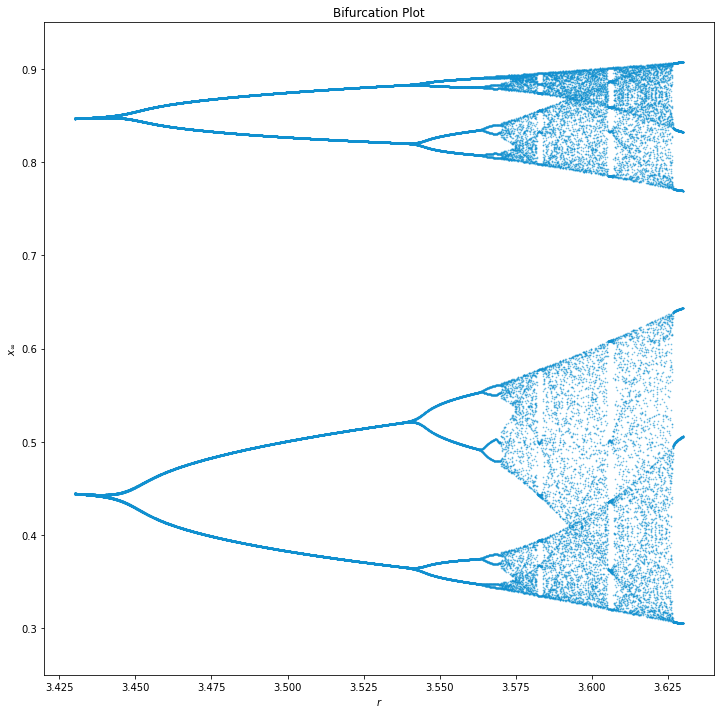
\includegraphics[width=.64\textwidth]{images/task4-1 zoom.png}
    \caption{Zoomed-in bifurcation results for $r\in[3.43, 3.63]$, where the bifurcation of stable values into branches and chaos can be observed}
    \label{fig:task4-1-zoom}
\end{figure}

Within the part of chaotic behavior, we can still observe that the bifurcation diagram on several isolated islands of $r$ values becomes sparse and yields oscillation again. The following result near $r=3.84$ (Figure \ref{fig:task4-1-3}) shows a case where the series briefly returns to an oscillation between 3 values.

\begin{figure} [H]
    \centering
    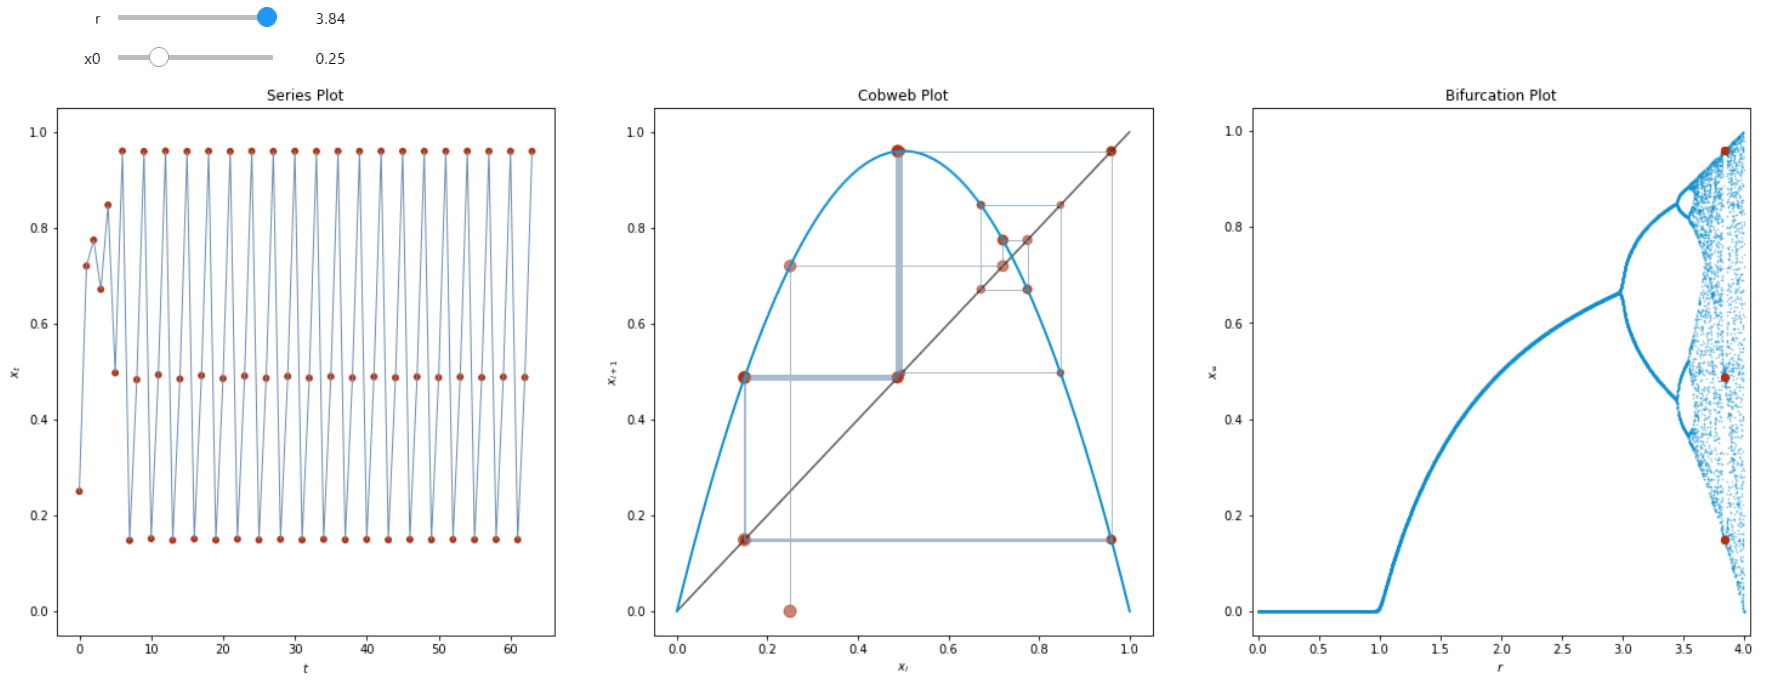
\includegraphics[width=.7\textwidth]{images/task4-1 (7).png}
    \caption{Results of $r=3.84$, with $x_0=0.25$}
    \label{fig:task4-1-3}
\end{figure}

We also plot the result of changing $x_0$ value for different $r$, and discovered that for the cases of $r$ where the series approach one value or oscillation among various values, the initial conditions has not effect of the final results; and for the chaos part a slight change in $x_0$ would lead to drastically different results in the plots, which by definition shows the feature of chaotic behaviors.

\begin{figure} [H]
    \centering
    \subfloat[$r=3.20, x_0=0.05$]{
        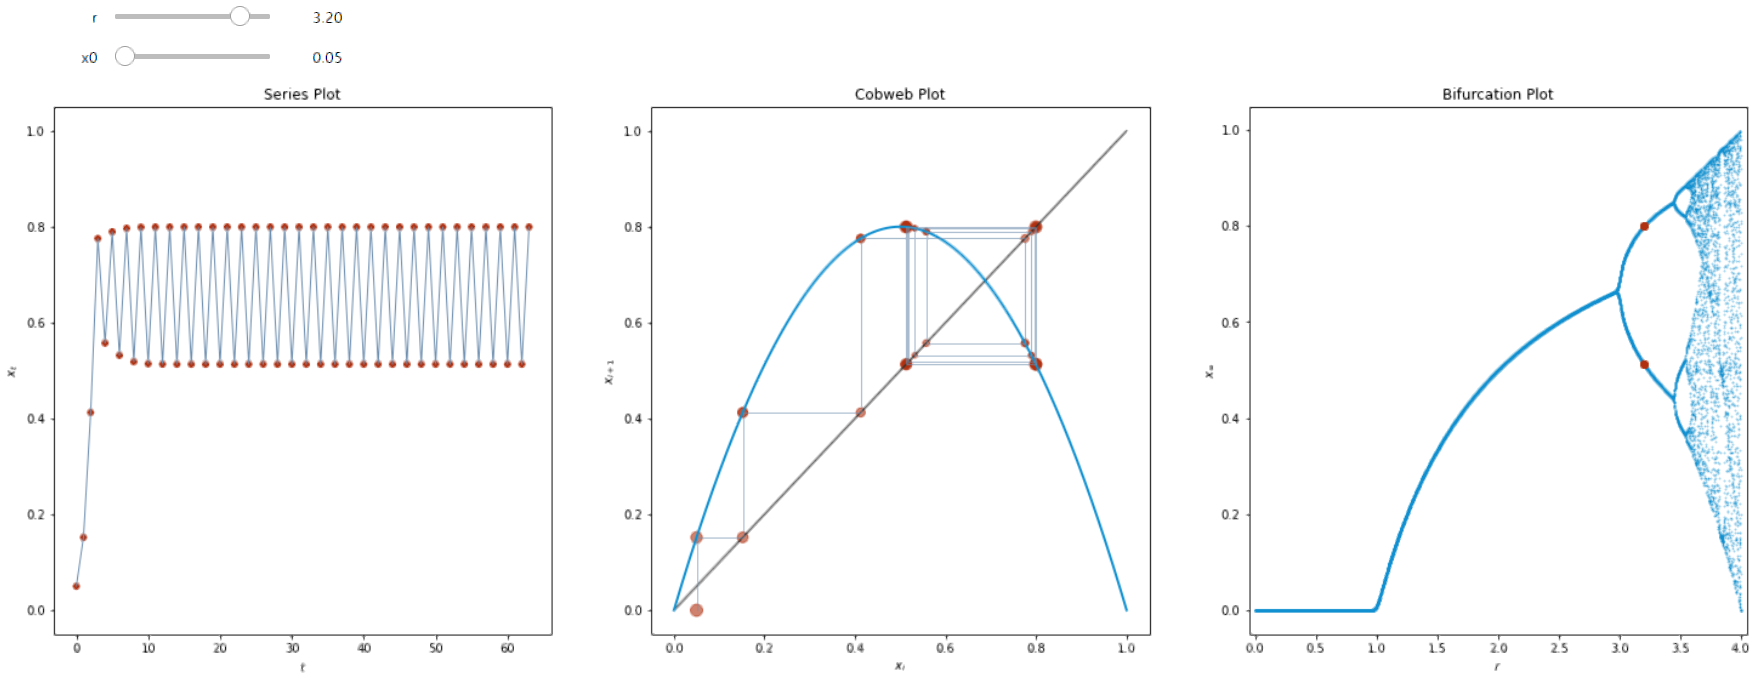
\includegraphics[width=.7\textwidth]{images/task4-1 x0-1.png}}
    \\
    \subfloat[$r=3.20, x_0=0.85$]{
        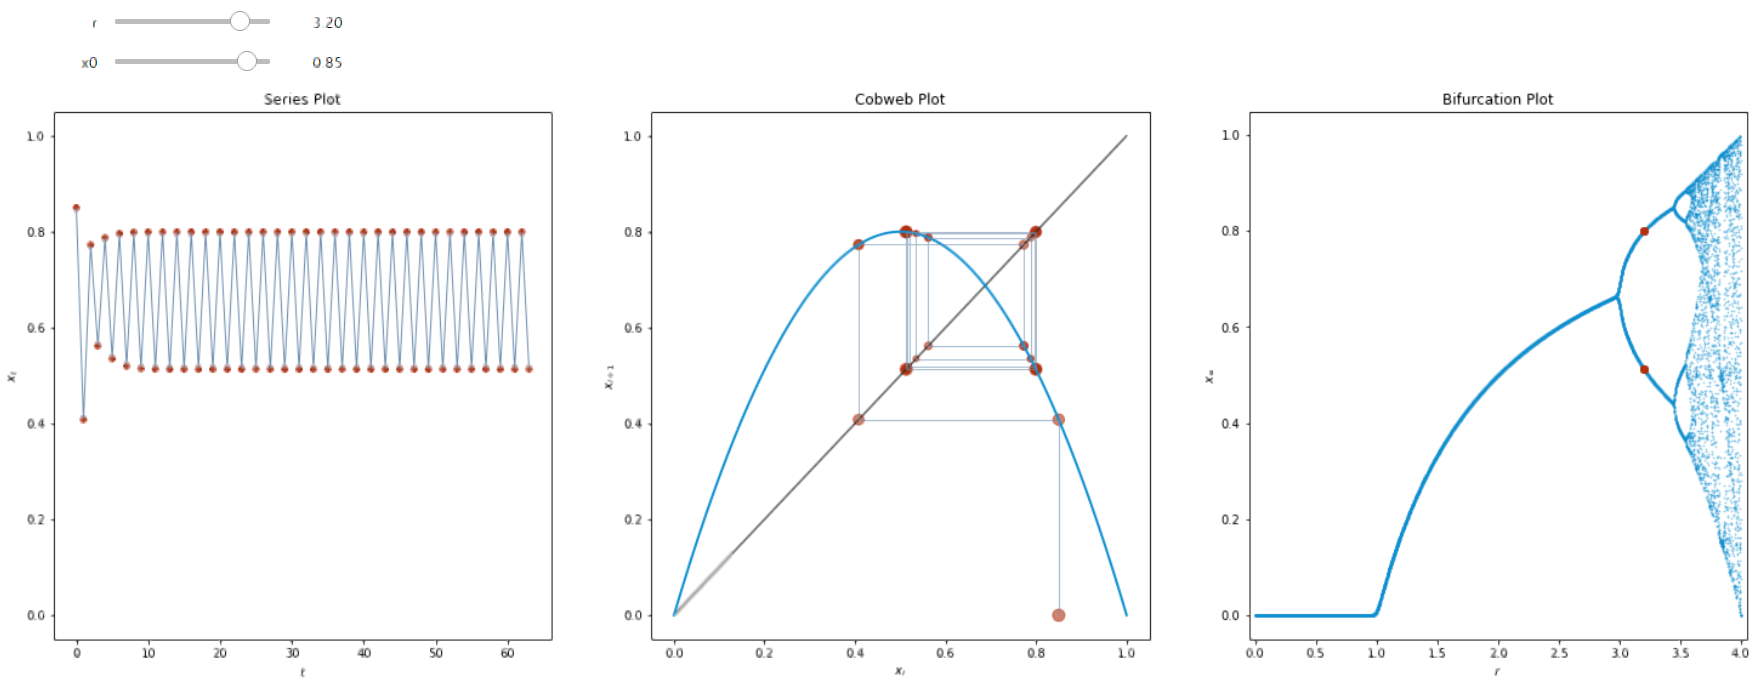
\includegraphics[width=.7\textwidth]{images/task4-1 x0-2.png}}
    \\
    \subfloat[$r=3.80, x_0=0.05$]{
        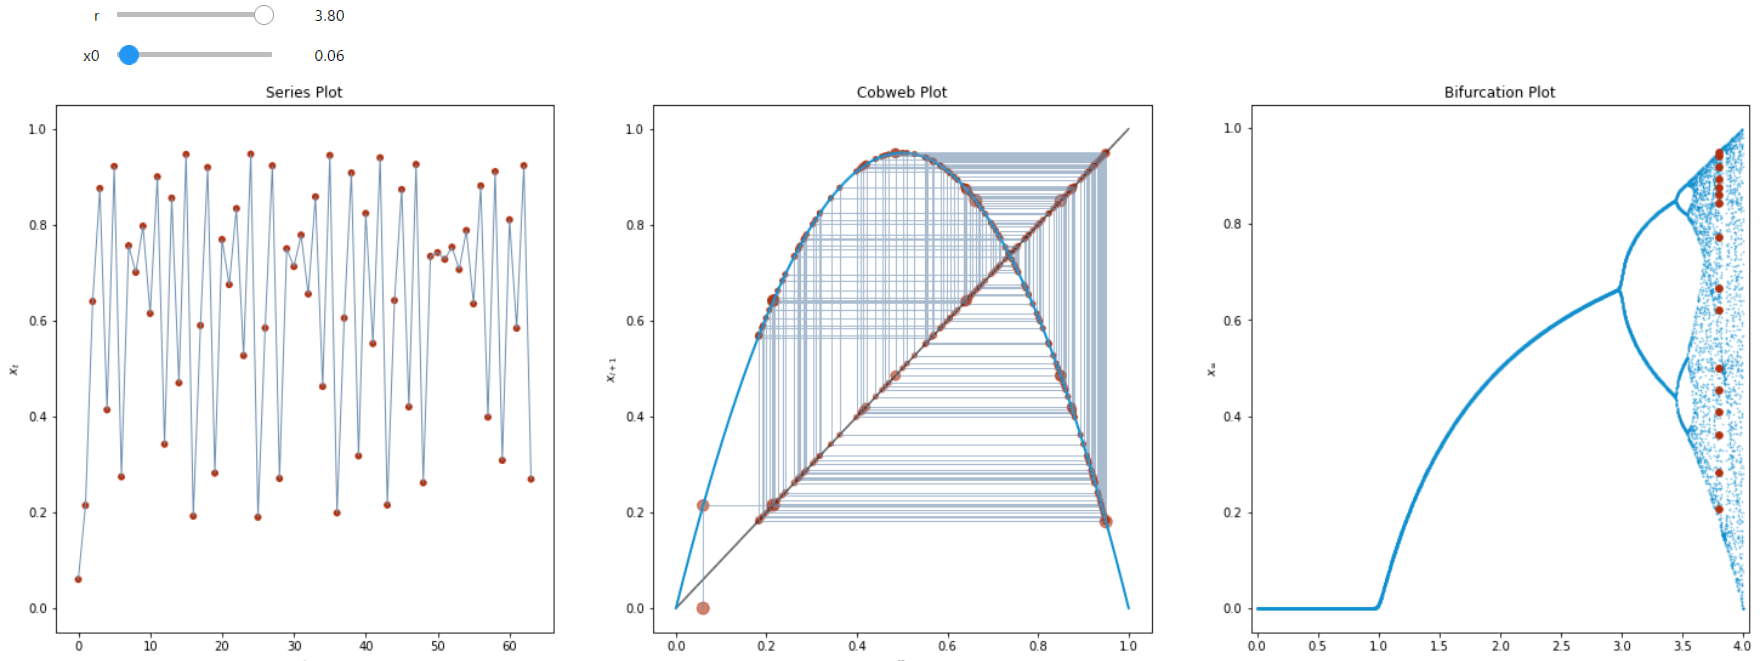
\includegraphics[width=.7\textwidth]{images/task4-1 x0-3.png}}
    \\
    \subfloat[$r=3.80, x_0=0.06$]{
        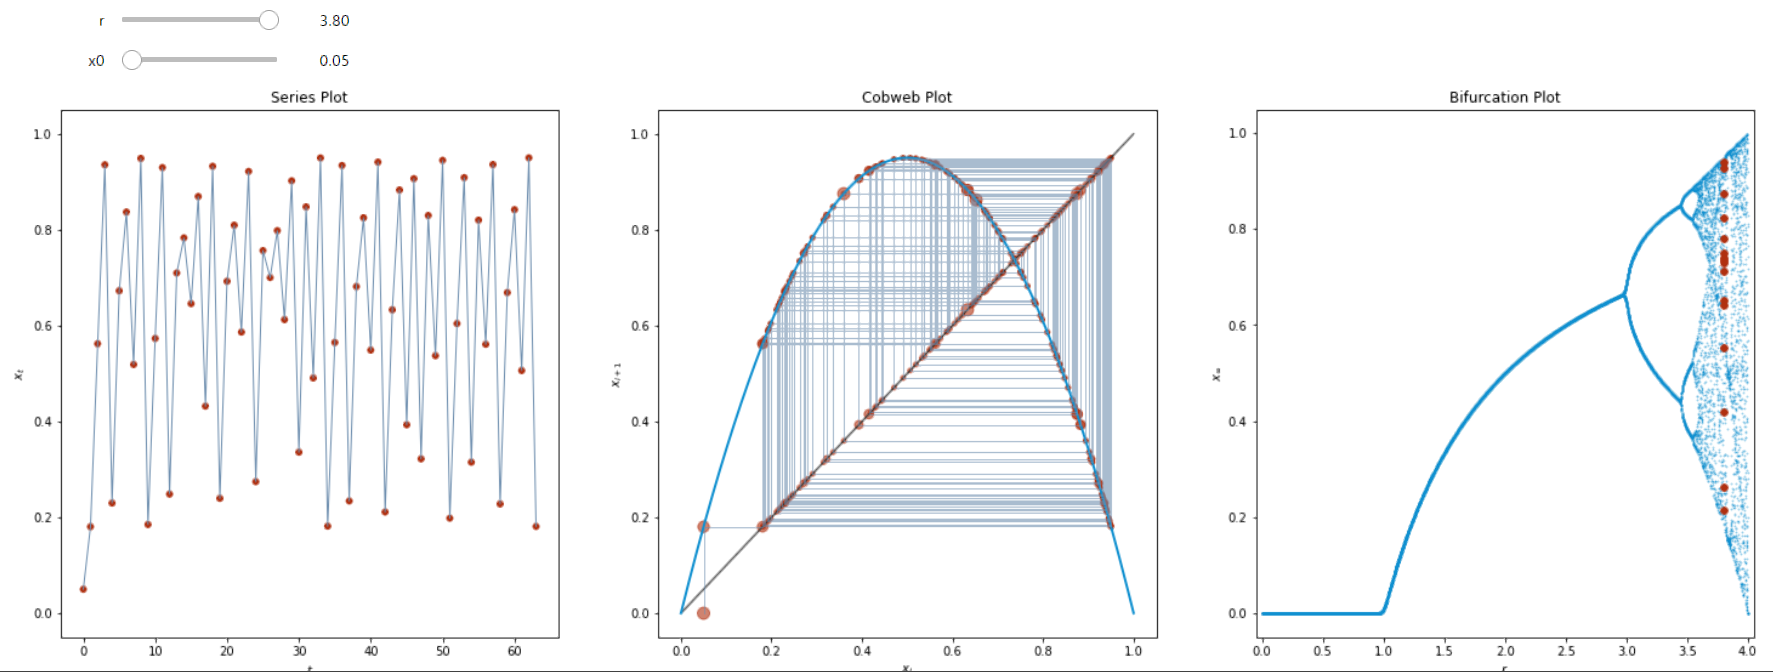
\includegraphics[width=.7\textwidth]{images/task4-1 x0-4.png}}
    \caption{Varying $x_0$ has different effect depending on $r$}
    \label{fig:task4-1-x0}
\end{figure}

\newpage

\noindent \textbf{Part 2:} 

Now we study the Lorenz attractor as a dynamical system in continuous time with smooth evolution operators that produce chaotic dynamics when the dimension of the state space is larger than 2. The system can be defined as
\begin{align}
    \dot{X} &= -\sigma X + \sigma Y,\\
    \dot{Y} &= -XZ+\rho X-Y,\\
    \dot{Z} &= XY-\beta Z
\end{align}
in which $X, Y, Z$ denotes the 3-dimensional coordinates of the system, dot denotes the derivative with respect to the dimensionless time, while $\sigma, \rho, \beta$ are the system parameters.

\begin{lstlisting}[language = Python,  label = {cusp_method}]
def lorenz(x, y, z, s=10, b=8/3, r=28):
    ''' 
    Definition of the derivative equation for the lorenz system.
    :param x, y, z: float
        current system value
    :param s, b, r: float
        lorenz model parameters
    :returns: float
        derivative result of x, y, z
    '''
    dx = s*(y - x)
    dy = r*x - y - x*z
    dz = x*y - b*z
    return dx, dy, dz
\end{lstlisting}

For simulating and visualizing the trajectory of a point through time within this system, we iteratively calculate the derivative value at current location, multiply by $\text{d}t$ and add it to the current location, and use this new location for calculating in the next iteration, until the simulation reached the termination time $T_\text{end}$.

\begin{lstlisting}[language = Python,  label = {cusp_method}]
def visualize(Tend, x0, y0, z0, s, b, r):   
    '''
    Calculate and plot the 3D trajectory of the Lorenz model from the initial state x_0=(x0, y0, z0), 
    and parameters sigma=s, beta=b, rho=r, simulating within range of time from 0 to Tend.
    Results given by updating calculated coordinates of the points on the bifurcation plot
    into global lists xs_record and ys_record.

    :param Tend: int
        Termination time of the simulation 
    :param x0, y0, z0: float
        initial state value
    :param s, b, r: float
        lorenz model parameters
    :returns: none
    '''
    # Define the time step size and number of iterations
    dt = 0.01
    num_iterations = int(Tend / dt)

    # Set up the arrays to store the values of x, y, and z
    x = np.empty(num_iterations + 1,)
    y = np.empty(num_iterations + 1,)
    z = np.empty(num_iterations + 1,)

    # Set the initial values of x, y, and z
    x[0], y[0], z[0] = (x0, y0, z0)
    # Iterate over the time steps and update the values of x, y, and z using the Lorenz system equations
    for i in range(num_iterations):
        dx, dy, dz = lorenz(x[i], y[i], z[i], s, b, r)
        if (dx>1e8 or dy>1e8 or dz>1e8):
            break
        x[i + 1] = x[i] + dx * dt
        y[i + 1] = y[i] + dy * dt
        z[i + 1] = z[i] + dz * dt

    # Set up the 3D plot and draw the trajectory of the Lorenz system
    fig = plt.figure(figsize=(10,10))
    ax = fig.add_subplot(111, projection='3d')
    ax.plot(x[:i], y[:i], z[:i], lw=min(0.8, 80/Tend))
    ax.set_xlabel("X Axis")
    ax.set_ylabel("Y Axis")
    ax.set_zlabel("Z Axis")
    plt.show()
\end{lstlisting}

To better demonstrate our result, we also designed interactive user interface to dynamically change the $Tend$ value, initial location and model parameters. The result for $x_0=(10, 10, 10), \sigma=10, \beta=8/3, \rho=28$ is shown in figure \ref{fig:task4-2-1}.

\begin{figure} [H]
    \centering
    \subfloat[$T_\text{end}=25$]{
        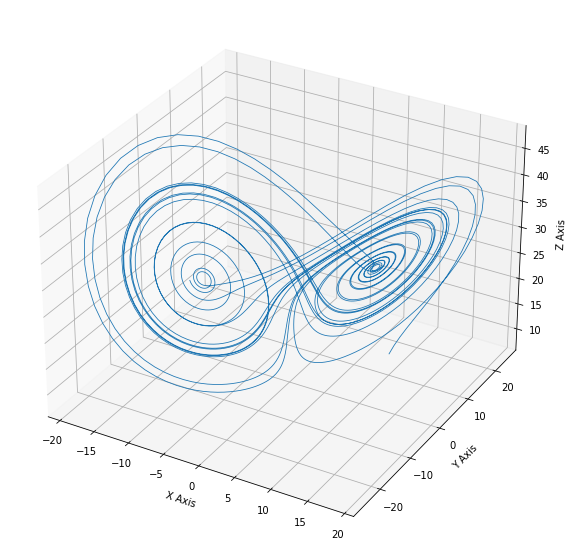
\includegraphics[width=.3\textwidth]{images/task4-2-1-25.png}}
    \subfloat[$T_\text{end}=200$]{
        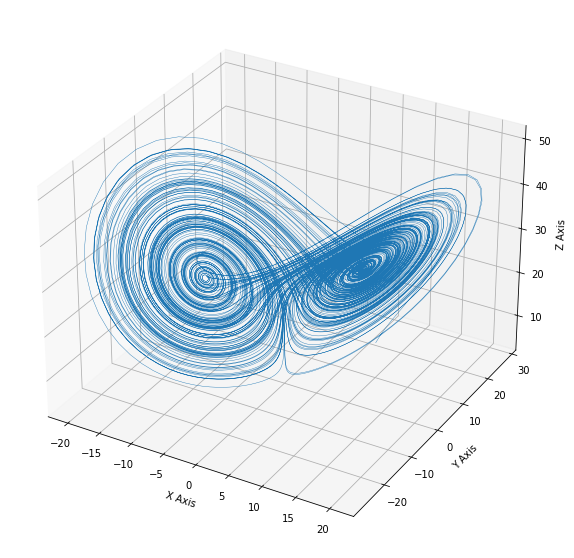
\includegraphics[width=.3\textwidth]{images/task4-2-1-200.png}}
    \subfloat[$T_\text{end}=1000$]{
        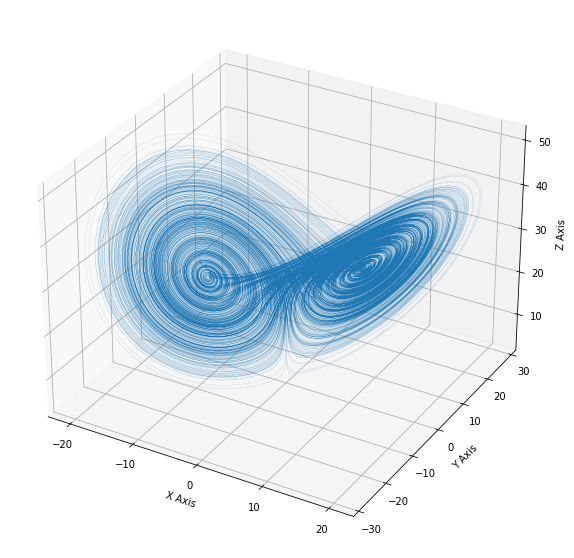
\includegraphics[width=.3\textwidth]{images/task4-2-1-1000.png}}
    \caption{Simulated trajectory of the Lorenz system starting at $x_0=(10, 10, 10)$, with parameter values $\sigma=10, \beta=8/3, \rho=28$}
    \label{fig:task4-2-1}
\end{figure}

The simulated result above shows the distinctive ``butterfly'' shape of a typical Lorenz system.

The behavior of the Lorenz attractor is sensitive to initial conditions, implying that small perturbations in the starting values of the variables can result in significantly different outcomes over time. This sensitivity to initial conditions, also known as the butterfly effect, is one of the key features of chaotic systems. To test this we plot another trajectory from $\hat{x}_0=(10+10^{-8}, 10, 10)$ and separately another plot for the difference between two trajectories $||x(t)-\hat{x}(t)||^2$ over time. To do this, we modify the previous function:

\begin{lstlisting}[language = Python,  label = {cusp_method}]
def compare(Tend=1000, x0=10, y0=10, z0=10, s=10, b=8/3, r=28):   
    ...
    # Set the initial values of x, y, and z
    x[0], y[0], z[0] = (x0, y0, z0)
    x_hat[0], y_hat[0], z_hat[0] = (x0+(1e-8), y0, z0)

    # Iterate over the time steps and update the values of x, y, and z using the Lorenz system equations
    for i in range(num_iterations):
        dx, dy, dz = lorenz(x[i], y[i], z[i], s, b, r)
        dx_hat, dy_hat, dz_hat = lorenz(x_hat[i], y_hat[i], z_hat[i], s, b, r)
        if (dx>1e8 or dy>1e8 or dz>1e8 or dx_hat>1e8 or dy_hat>1e8 or dz_hat>1e8):
            break
        x[i + 1] = x[i] + dx * dt
        y[i + 1] = y[i] + dy * dt
        z[i + 1] = z[i] + dz * dt
        x_hat[i + 1] = x_hat[i] + dx_hat * dt
        y_hat[i + 1] = y_hat[i] + dy_hat * dt
        z_hat[i + 1] = z_hat[i] + dz_hat * dt
    
    distance = np.sqrt((x - x_hat)**2 + (y - y_hat)**2 + (z - z_hat)**2)

    # Set up the 3D plot and draw the trajectory of the Lorenz system
    fig = plt.figure(figsize=(20,10))
    ax1 = fig.add_subplot(121, projection='3d')
    ax1.plot(x[:i], y[:i], z[:i], color='blue', lw=min(0.5, 50/Tend))
    ax1.plot(x_hat[:i], y_hat[:i], z_hat[:i], color='red', lw=min(0.5, 50/Tend))
    ax1.set_xlabel("X Axis")
    ax1.set_ylabel("Y Axis")
    ax1.set_zlabel("Z Axis")
    
    # Plot the distance between the coordinates and the fixed point in the second subplot
    ax2 = fig.add_subplot(122)
    ax2.plot(distance, lw=0.5)
    ax2.set_xlabel("Time Step")
    ax2.set_ylabel("Distance")
    ax2.set_xlim(xmin=0, xmax=i)
    
    plt.show()
\end{lstlisting}

\begin{figure} [H]
    \centering
    \subfloat[$T_\text{end}=15$]{
        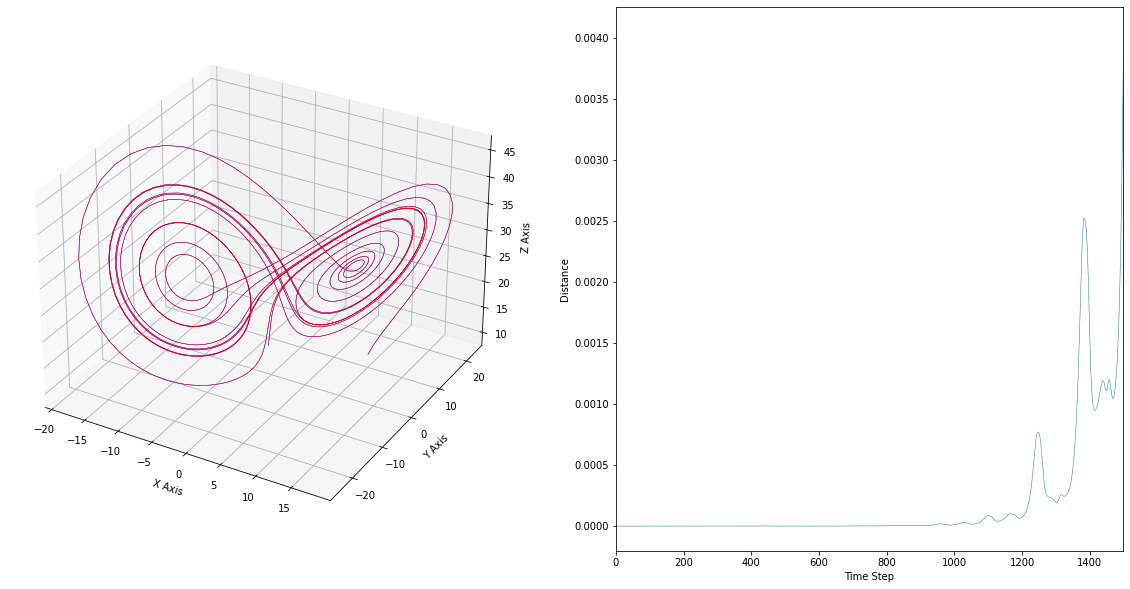
\includegraphics[width=.6\textwidth]{images/task4-2-2-15.png}}
    \\
    \subfloat[$T_\text{end}=25$]{
        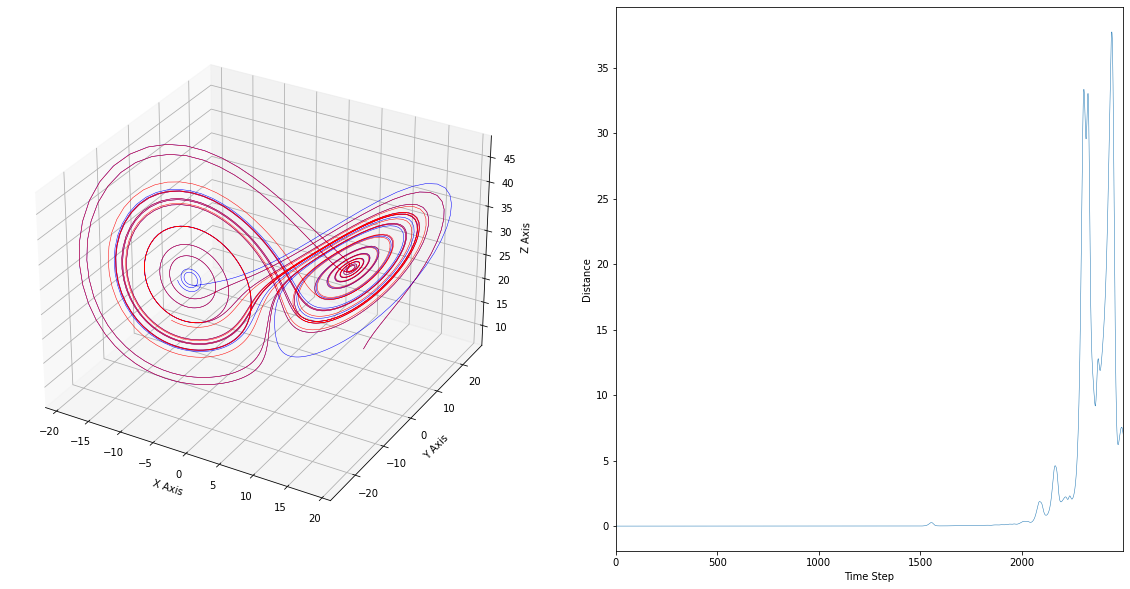
\includegraphics[width=.6\textwidth]{images/task4-2-2-25.png}}
    \\
    \subfloat[$T_\text{end}=100$]{
        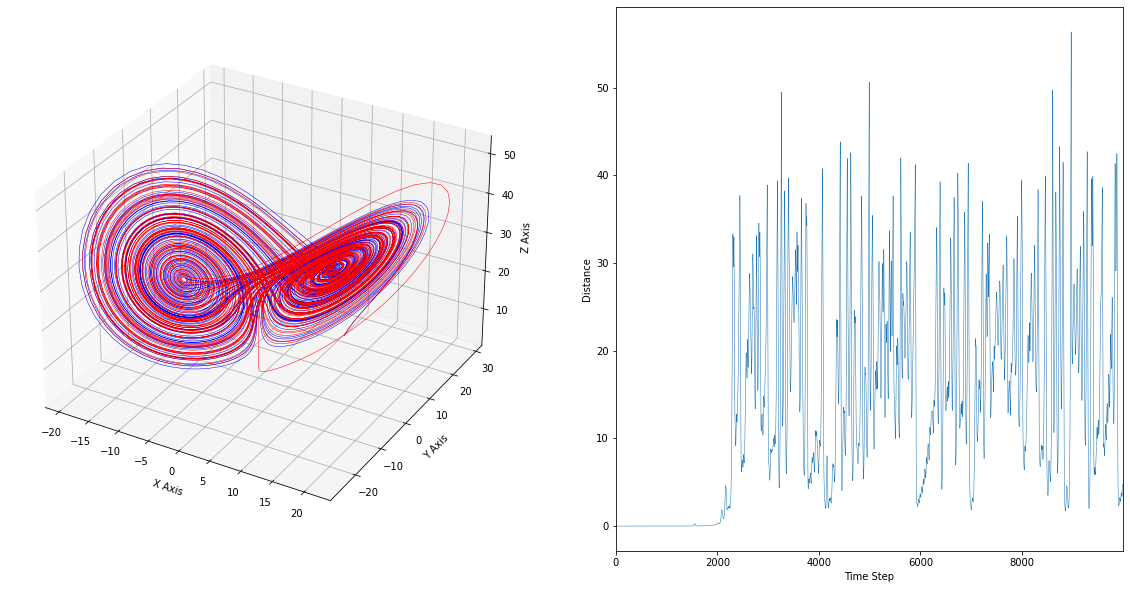
\includegraphics[width=.6\textwidth]{images/task4-2-2-100.png}}
    \caption{Simulated trajectories of the Lorenz system and the distance in between, starting at $x_0=(10, 10, 10)$ and $\hat{x}_0=(10+10^{-8}, 10, 10)$, with parameter values $\sigma=10, \beta=8/3, \rho=28$}
    \label{fig:task4-2-2}
\end{figure}

Two trajectories starting from initial states that are very close ($10^{-8}$) has shown to keep the small distance at the beginning, whereas we can observe that the distance is getting larger as $T$ increases. After $T_\text{end}>20$, the distance between the points on the trajectory turns larger than 1. And we can see the derivation clearly at $T_\text{end}=25$, where two trajectories are ending at different sides of wing of the attractor, and the difference becomes as large as the diameter of the attractor. Further increasing $T$, the difference value turns into chaotic fluctuation between 0 and 60.

Now we change the parameter value $\rho$ into different values, and compute and plot the two trajectories.

\begin{figure} [H]
    \centering
    \subfloat[$\rho=0.5$]{
        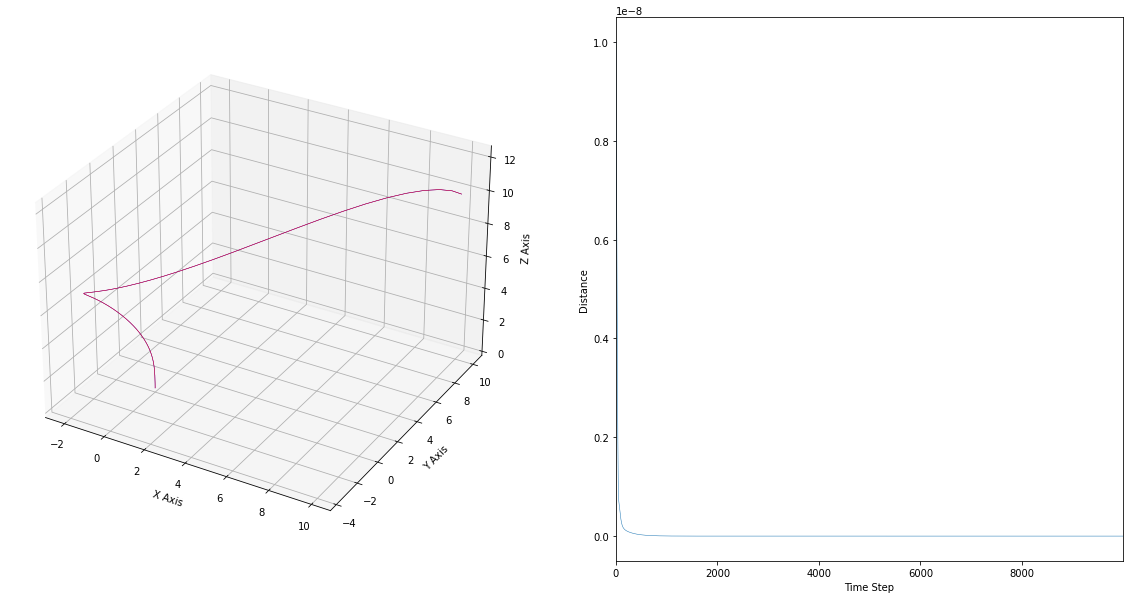
\includegraphics[width=.5\textwidth]{images/task4-2-2-r-0.5.png}}
    \subfloat[$\rho=5$]{
        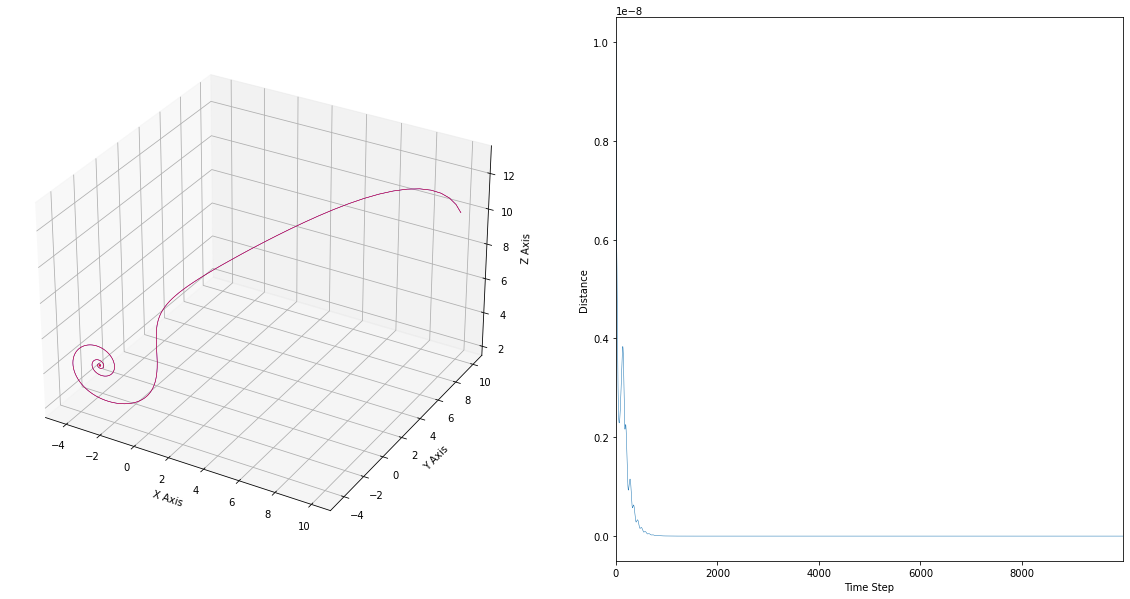
\includegraphics[width=.5\textwidth]{images/task4-2-2-r-5.png}}
    \\
    \subfloat[$\rho=10$]{
        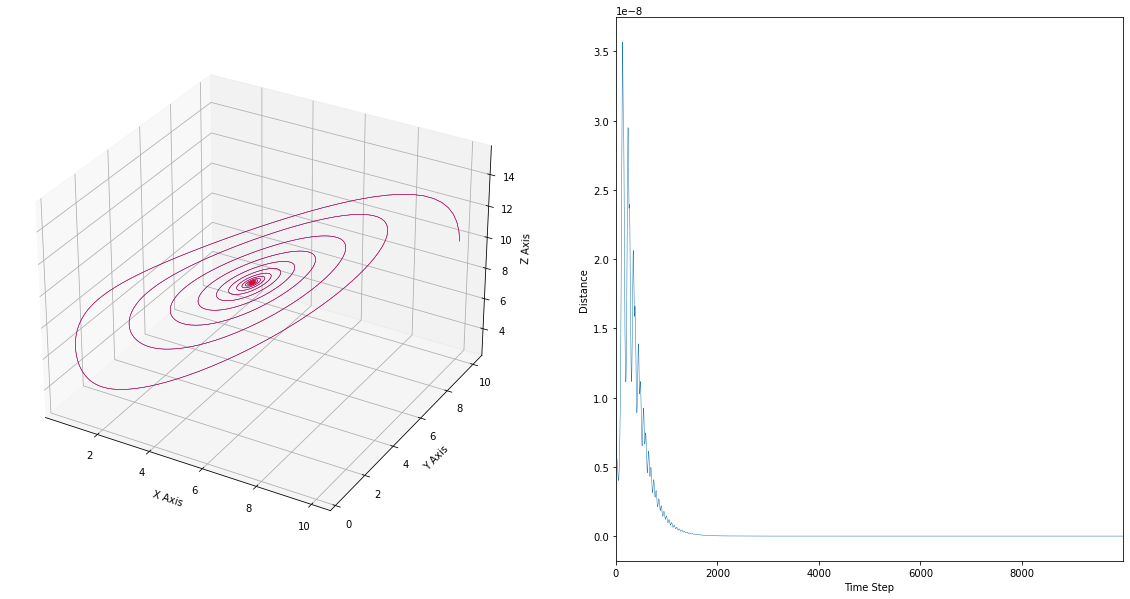
\includegraphics[width=.5\textwidth]{images/task4-2-2-r-10.png}}
    \subfloat[$\rho=14$]{
        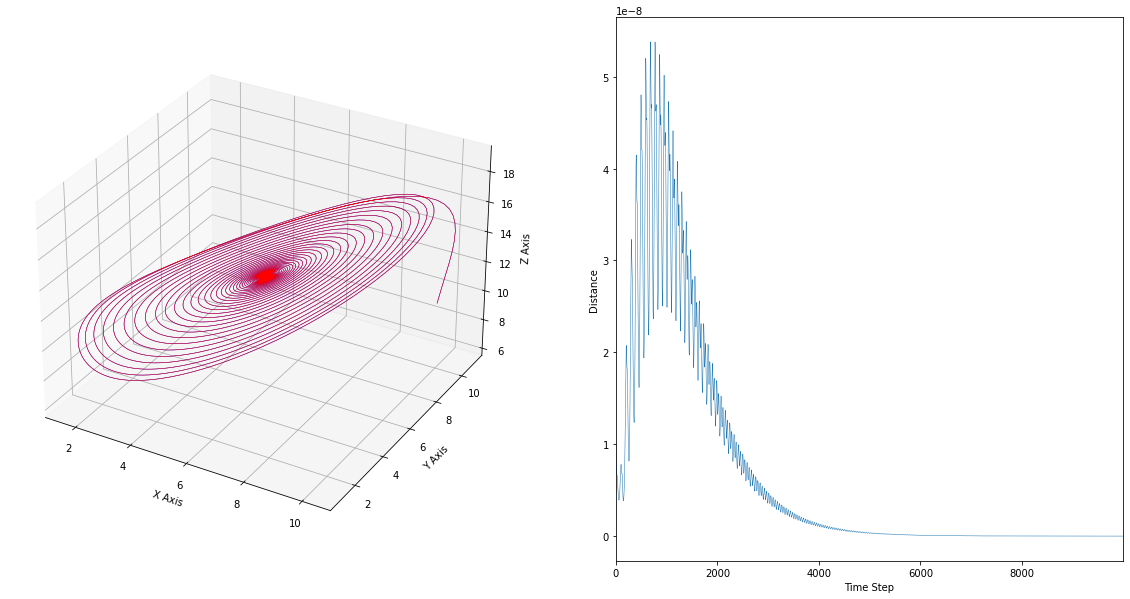
\includegraphics[width=.5\textwidth]{images/task4-2-2-r-14.png}}
    \\
    \subfloat[$\rho=15$]{
        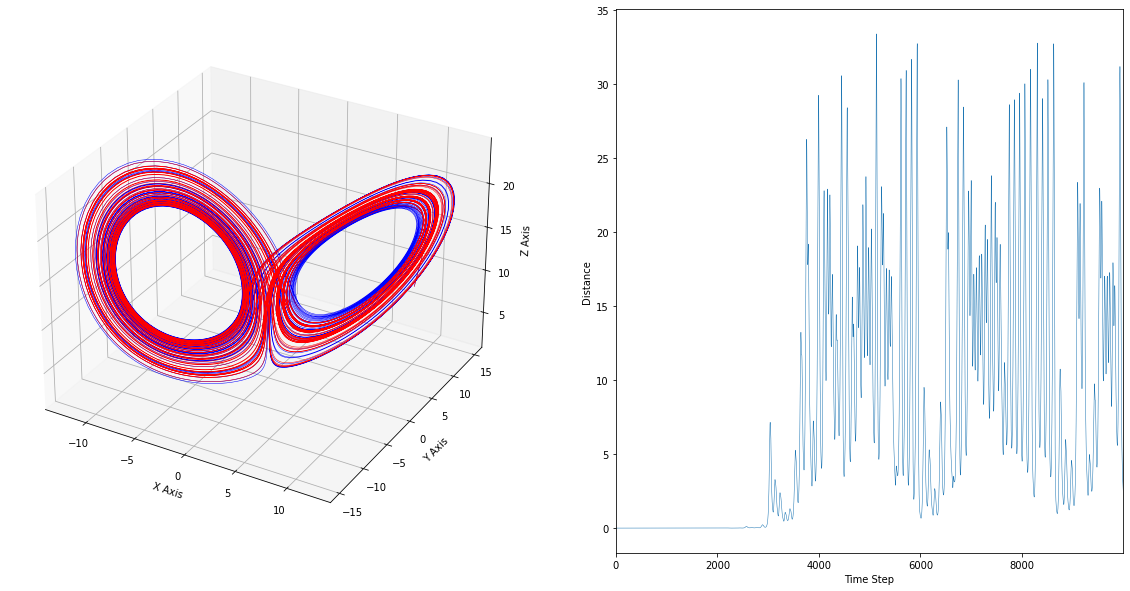
\includegraphics[width=.5\textwidth]{images/task4-2-2-r-15.png}}
    \subfloat[$\rho=40$]{
        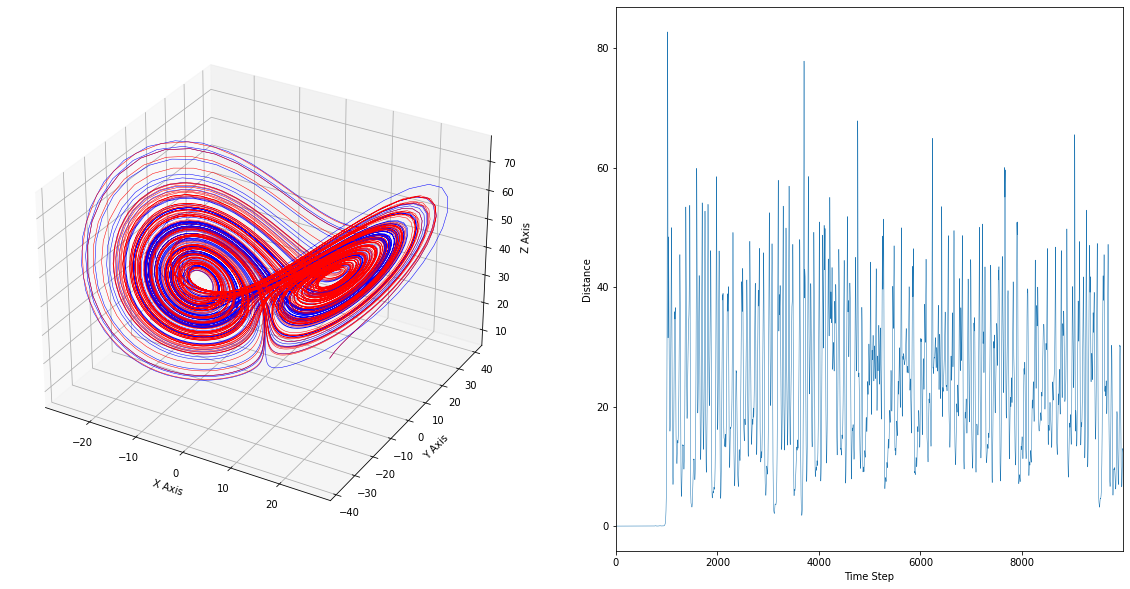
\includegraphics[width=.5\textwidth]{images/task4-2-2-r-40.png}}
    \caption{Simulated trajectories of the Lorenz system and the distance in between, starting at $x_0=(10, 10, 10)$ and $\hat{x}_0=(10+10^{-8}, 10, 10)$, with parameter values $\sigma=10, \beta=8/3$ and terminal time $T_\text{end}=100$}
    \label{fig:task4-2-r}
\end{figure}

For $\rho=0.5$, the two trajectories all end at a same value very quickly, and stayed there after $T=1$. No bifurcation happens for this value of $\rho$. Same goes for all $\rho<=14$, where the trajectories eventually end at one fixed point attractor and leading the difference shrink to 0. The bifurcation happens after approximately $\rho=14.54$, where the fixed points become repulsors and the trajectory is repelled by them in a very complex way, and keep this chaotic feature for all larger $\rho$. This bifurcation point is relative to the initial location of the system, for example if we take $x_0=(0.1,0.1,0.1)$, the bifurcation would happen at $\rho=15.20$.

We also plotted a bifurcation diagram of how distance changes for different $\rho$. Already knowing that bifurcation happens at $\rho=14.54$ for the given $x_0$ and other parameters, we hereby only calculate the result for 800 different $\rho$ values in between $[14.50, 14.60]$. The bifurcation between two different behaviours can be observed clearly through figure \ref{fig:task4-2-b}. 

\begin{figure} [H]
    \centering
    \subfloat{
        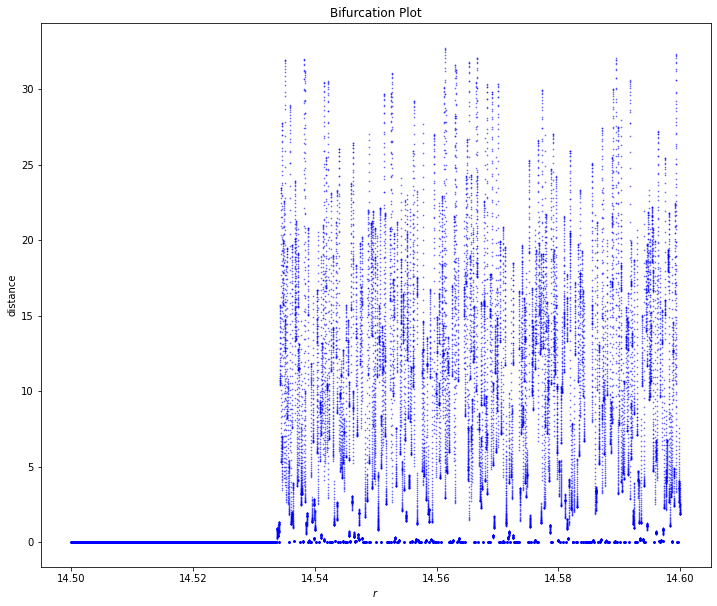
\includegraphics[width=.7\textwidth]{images/task4-2-2-r-bifurc.png}}
    \caption{Bifurcation result of the distance in between two trajectories starting at $x_0=(10, 10, 10)$ and $\hat{x}_0=(10+10^{-8}, 10, 10)$, with parameter values $\sigma=10, \beta=8/3$ and terminal time $T_\text{end}=50$, varying agains different $\rho\in [14.50, 14.60]$}
    \label{fig:task4-2-b}
\end{figure}

\bigskip

\end{task}

\newpage

\begin{task}{5, Bifurcations in crowd dynamics }

In this last task, we have to apply our knowledge about bifurcation theory to analyze and describe a given SIR model. To complete the task, we done the following:

\bigskip

\noindent \textbf{Subtasks 1 - 2:} 

First of all we have download the unfinished SIR bed model from Moodle. The model is incomplete since it does not implement the differential equations and also it is not very well-documented, so we have implemented the equations in the \textit{sirModel.py} and added the missing documentation of the model. 

\begin{equation}\label{dS}
    \frac{dS}{dt} = A - \delta S - \frac{\beta S I}{S + I + R}
\end{equation}

\begin{equation}\label{dI}
    \frac{dI}{dt} = -(\delta + \upsilon)I - \mu(b,I)I + \frac{\beta S I}{S + I + R}
\end{equation}

\begin{equation}\label{dR}
    \frac{dR}{dt} = \mu(b,I)I - \delta R
\end{equation}

The equations \ref{dS}, \ref{dI} and \ref{dR} are the differential equation and below we can observe their code implementation on \textit{sirModel.py}:

\begin{lstlisting}[language = Python, label={decoupling}]

def model(t, y, mu0, mu1, beta, A, d, nu, b):
    """
    SIR model including hospitalization and natural death.
    
    Parameters:
    -----------
    mu0
        Minimum recovery rate
    mu1
        Maximum recovery rate
    beta
        average number of adequate contacts per unit time with infectious individuals
    A
        recruitment rate of susceptibles (e.g. birth rate)
    d
        natural death rate
    nu
        disease induced death rate
    b
        hospital beds per 10,000 persons
    """
    S,I,R = y[:]
    m = mu(b, I, mu0, mu1)
    
    dSdt = A - d * S - (beta * S * I) / (S + I + R)
    dIdt = - (d + nu) * I - m * I + (beta * S * I) / (S + I + R)
    dRdt = m * I - d * R
    
    return [dSdt, dIdt, dRdt]
    
\end{lstlisting}

As we can see, all the parameters needed are passed as parameters of the function, so it was quite straight forward to implement those equations. 

We have also renamed the notebook as \texttt{Task5.ipynb} and moved the code snippet to plot the system's trajectories and the behaviour of the S, I and R variables over time (Figure \ref{task5_1}) to \textit{sirModel.py} to make the code more modular and concise.

\begin{figure} [H]
    \centering
    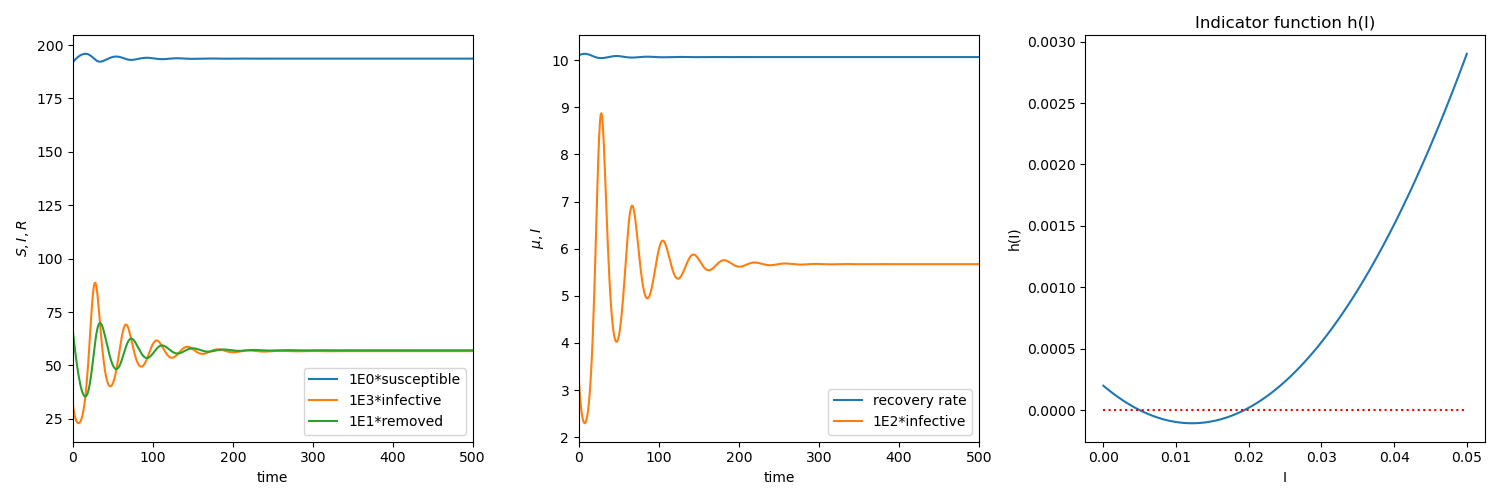
\includegraphics[width=15cm]{images/Task1.png}
    \caption{SIR variables over time, recovery rate VS infective variable and indicator function for bifurcations (from left to right)}
    \label{task5_1}
\end{figure}

\noindent \textbf{Subtask 3:} 

The parameters for this parts are already set, and we have only changed the parameter b in order to see a special bifurcation. Among the 20 plots generated for the parameter b in the range of [0.01, 0.03] in steps of 0.001, we have selected nine of them, as it can be seen in the Figure \ref{plots}. The three starting points of those plots are:

\begin{itemize}
  \item SIR point 1: [195.3 0.052 4.40], its trajectory is colored in red.
  \item SIR point 2: [195.7 0.030 3.92], its trajectory is colored in blue.
  \item SIR point 3: [193.0 0.080 6.21], its trajectory is colored in green.
\end{itemize} 

\noindent {By varying the parameter b, we can observe three different behaviours:}
\begin{itemize}
  \item b $<$ 0.022: the system shows a local attractive point (steady state) approximately around one point. As the value of the parameter b increases, it looks more likely to a stable focus around a point.
  \item b = 0.022: there is an equilibrium (bifurcation) point at this value of b. As we can observe in the plot of the SIR trajectory with b: 0.022, there is a weak stable point that is attracting the first point (red trajectory) and the other two points (blue and green trajectories) being attracted to a stable limit cycle.  
  \item b $>$ 0.022: the system converges once again. The new attractive steady state is ubicated around the point [200 0 0], which is the the disease free equilibrium point $E_0$. 
  
  $E_0 = (A/d, 0, 0) = (20/0.1, 0, 0) = (200, 0, 0)$
\end{itemize} 

\begin{figure} [H]
\begin{subfigure} {0.33\textwidth}
    \centering
    \label{task5-3-1}
    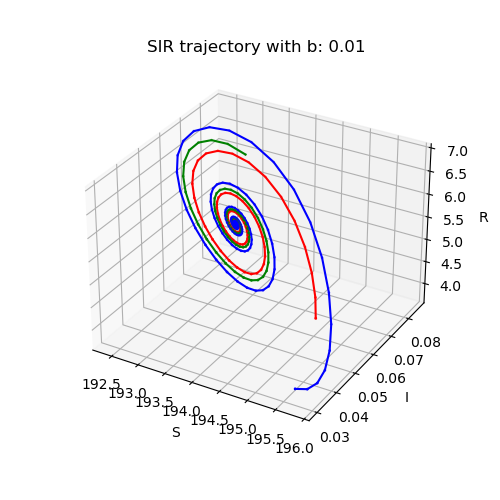
\includegraphics[width=.9\linewidth]{images/0.01.png} 
\end{subfigure}
\begin{subfigure} {0.33\textwidth}
    \centering
    \label{task5-3-2}
    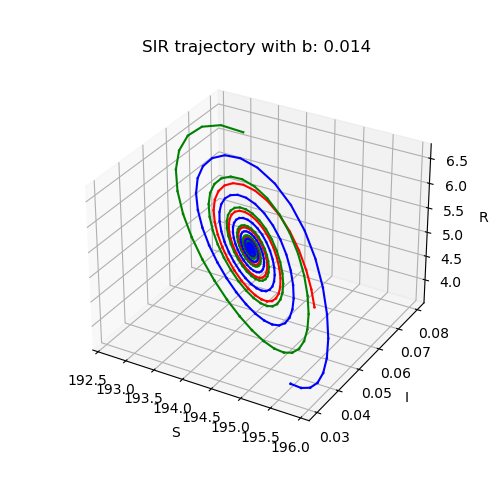
\includegraphics[width=.9\linewidth]{images/0.014.png} 
\end{subfigure}
\begin{subfigure} {0.33\textwidth}
    \centering
    \label{task5-3-3}
    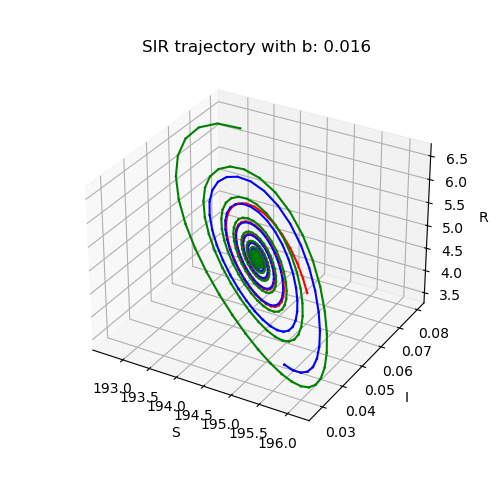
\includegraphics[width=.9\linewidth]{images/0.016.png} 
\end{subfigure}
\medskip
\begin{subfigure} {0.33\textwidth}
    \centering
    \label{task5-3-4}
    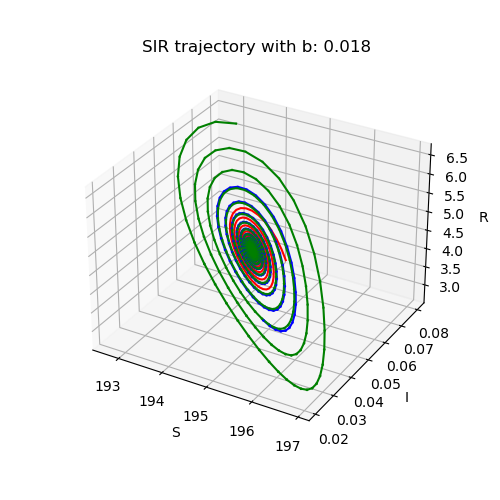
\includegraphics[width=.9\linewidth]{images/0.018.png} 
\end{subfigure}
\begin{subfigure} {0.33\textwidth}
    \centering
    \label{task5-3-5}
    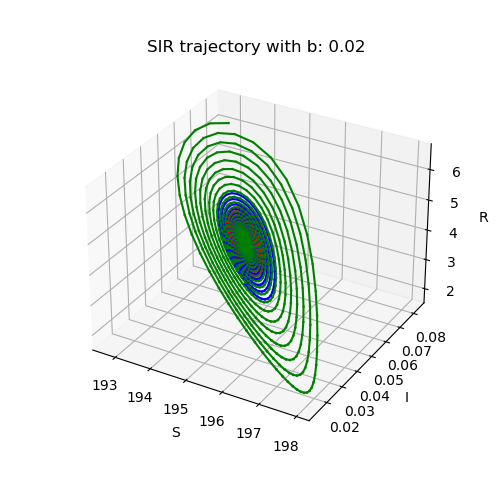
\includegraphics[width=.9\linewidth]{images/0.02.png} 
\end{subfigure}
\begin{subfigure} {0.33\textwidth}
    \centering
    \label{task5-3-6}
    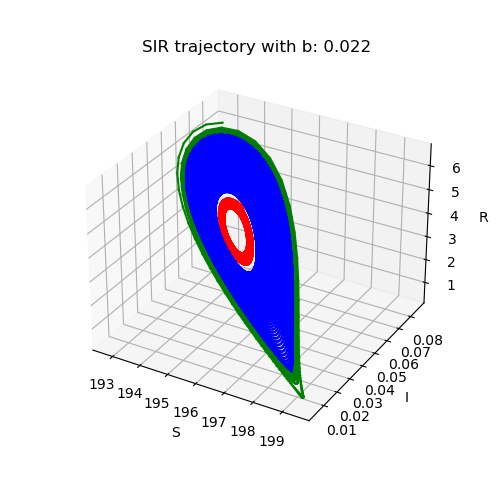
\includegraphics[width=.9\linewidth]{images/0.022.png} 
\end{subfigure}
\medskip
\begin{subfigure} {0.33\textwidth}
    \centering
    \label{task5-3-7}
    \includegraphics[width=.9\linewidth]{images/0.024.png} 
\end{subfigure}
\begin{subfigure} {0.33\textwidth}
    \centering
    \label{task5-3-8}
    \includegraphics[width=.9\linewidth]{images/0.026.png} 
\end{subfigure}
\begin{subfigure} {0.33\textwidth}
    \centering
    \label{task5-3-9}
    \includegraphics[width=.9\linewidth]{images/0.03.png} 
\end{subfigure}
    \caption{Trajectory of SIR variables by changing b - evolution from from left to right and up to down}
    \label{plots}
\end{figure}

\noindent \textbf{Subtask 4:} 

It is a Hopf Bifurcation that happens in the value b = 0.022, since the system is going from a local steady state to a limit cycle as we have described in the previous subtask 3. We can find the normal form of a Hopf Bifurcation in the section \textit{"3.4 The normal form of the Hopf bifurcation"} in the book of Kuznetsov \cite{Yuri} and it has the following form:
\begin{equation}\label{normalform1}
    \begin{split}
    & \dot{x}_1 = ax_1 - x_2 - x_1(x_1^2 + x_2^2) \\
    & \dot{x}_2 = x_1 + ax_2 - x_2(x_1^2 + x_2^2)
    \end{split}
\end{equation}

\newpage

\noindent \textbf{Subtask 5:} 

In this part, we have to analyse the reproduction rate $\mathbb{R}_0$ described in the next equation, that we can find in the section \textit{"3. Existence and types of equilibria"} in the book of Chunhua Shan and Huaiping Zhu \cite{Chunhua}: 

\begin{equation}\label{rr}
    \mathbb{R}_0 = \frac{\beta}{d + \upsilon + \mu_1}
\end{equation}

\noindent The variables used to compute the reproduction rate are:

\begin{itemize}
  \item $\beta$: represents the average number of adequate contacts per unit time with infectious individuals.
  \item d: represents the per capita natural death rate.
  \item $\upsilon$: represents the per capita disease-induced death rate.
  \item $\mu_1$: represents the maximum recovery rate based on the number of available beds.
\end{itemize} 

\noindent The reproduction rate indicates how the infection is spread among the population. The variable $\beta$ is in the numerator of the fraction, so if we increase or decrease this variable, it will have the same effect on $\mathbb{R}_0$ (increasing or decreasing it). 

\bigskip

\noindent \textbf{Subtask 6:} 

The affirmation "the disease free equilibrium $E_0$ = (A/d, 0, 0) at R0 $<$ 1 is an attracting node" of the Theorem 3.2 of \cite{Chunhua} means that for values of the SIR variables that are near to the free equilibrium point (A/d, 0, 0), the system will quickly reach that point and stays at it. This means, that the infection won't be spread through the population because the I component of the equilibrium point is 0.

As we have analysed in the subtask 3, for $b > 0.022$, the system always gets to $E_0$ no matter the point is close or far from $E_0$, while for $b < 0.022$ sometimes it is attracted by another local attractive point different from $E_0$, as it can be observed in the Figure \ref{plots}.  

\end{task}

\newpage
\begin{thebibliography}{9}
\bibitem{Yuri}
Yuri A. Kuznetsov. Elements of Applied Bifurcation Theory. Springer New York, 2004.
\bibitem{Chunhua}
Chunhua Shan and Huaiping Zhu. Bifurcations and complex dynamics of an SIR model with the impact of the number of hospital beds. Journal of Differential Equations, 257(5):1662–1688, September 2014.

\bibitem{Cusp}
John Guckenheimer and Yuri A. Kuznetsov (2007) Cusp bifurcation. Scholarpedia, {\url{http://www.scholarpedia.org/article/Cusp_bifurcation}}.

\end{thebibliography}


\bibliographystyle{plain}
\bibliography{Literature}

\end{document}